%This work was supported by the Institute of Systems Engineering, Macau University of Science and Technology.
%!TEX program 	= xelatex
\PassOptionsToPackage{quiet}{xeCJK}
\documentclass{format/MUSTThesisC}

% redeclare 
\newfontscript{CJK}{hani} 
% \newfontscript{CJK~Ideographic}{hani} 
\ExplSyntaxOff  
\usepackage{xeCJK}



\usepackage{amsmath,amssymb, amsfonts,amsthm}


\renewcommand{\figurename}{{Fig.}}
\renewcommand{\tablename}{{Table}}

%%%%%%%%%%%%%%%%%%%%%
%
% Here one can add any package whenever necessary
%
%%%%%%%%%%%%%%%%%%%%%%


\usetikzlibrary{arrows.meta,arrows,shapes,automata,backgrounds,petri,patterns,decorations.pathmorphing,positioning,calc,shapes.geometric}%插件
\usepackage{xcolor}
\usepackage{tcolorbox}
\usepackage{algorithmic}
\usepackage{diagbox}
\usepackage[ruled,vlined,linesnumbered]{algorithm2e}
\usepackage{tabu}

\usepackage{hyperref}
\hypersetup{
    colorlinks=true,
    linkcolor=black,
    filecolor=magenta,      
    urlcolor=blue,
    pdftitle={Overleaf Example},
    pdfpagemode=FullScreen,
    }

%\usepackage{xeCJK}

\begin{document}





% -------------------------------------------------<< 增加 MUST 校徽水印-----論文終稿使用

\AddToShipoutPicture{\BackgroundPic}

% The watermark line can be commented out when editing. After the thesis is done, one can recover this line such that the watermark is exposed (若水印影响编辑可先注释掉,完成后在加水印).

%% -------------------------------------------------<< 自動生成 MUST 指定格式的扉頁
\def\Ctitle 		{論文標題}
\def\Etitle 		{Thesis title}
\def\Sname 			{王茗琛}
\def\Sno 			{2230025907}
\def\Sfaculty 		{創新工程學院}
\def\Sprogram 		{智能技術碩士}
\def\Smajor 		{智能技術碩士}
\def\Ssupervisor	{劉新}
\def\Sdate			{YYYY/MM/DD}

% 自動生成論文扉頁
\mustTitle



%% -------------------------------------------------<< \mustCabstract 生成中文摘要
\mustCabstract
{
	% 引用目錄下的文件內容
	離線手寫簽名驗證是生物特徵技術的一個應用场景, 其根據用戶提供的手寫簽名与資料庫中該用戶存儲的手寫簽名進行對比以驗證用戶身份, 在日常生活中被廣泛用於安全認證, 金融交易等安全領域. 學術研究中, 離線手寫簽名驗證定義為作者獨立和作者依賴任務. 第一種任務是將手寫簽名與對應作者的參考簽名進行對比驗證. 第二種任務是在作者依賴任務的基礎上使用獨立的作者分類器判斷輸入簽名是否是偽造的.

本工作内容如下: 1. 提出圖像多尺度融合特徵的OSVTF端到端模型結構,初步驗證模型架構性能. 2. 針對多尺度特徵融合和模型優化部分, 進行消融實驗以證實模型子網絡組合方案的性能. 3. 針對作者依賴任務,將對比支持向量機或全局平均池化作爲分類器的OSVTF性能.

在實驗部分, OSVTF模型在BHSig-B 80/20數據集的作者獨立和作者依賴任務中EER為4.54\%和2.13\%, 在BHSig-H 100/60數據集的EER為3.90\%和2.68\%. 在消融實驗部分, OSVTF在CEDAR 50/5數據集的作者獨立任務中EER為4.75\%. 結果證實采取了多尺度融合特徵的OSVTF能夠加强對僞造簽名的敏感部分特徵學習, 部分優化將加快模型訓練過程的收斂速度.


% 本文研究離散事件繫統的監督控制問題。
% 在使用該範本中有任何問題請聯繫覃濤
% \href{mailto:zhwli@ieee.org}{zhwli@ieee.org}。
% 澳門科技大學系統工程研究所感謝覃濤對設計此範本的貢獻。


% \medskip\medskip

% The template can be used in online and offline ways. For the former (highly recommended), 
% Overleaf (\url{https://www.overleaf.com}) is a collaborative cloud-based LaTeX editor used for writing, editing and publishing scientific documents, which is much easy to use and friendly. In overleaf, the compiling command is \textcolor{blue}{XeLatex}.

% For the latter, one can use Texstudio, which is a very popular yet free software package (\url{https://www.texstudio.org/}). When using Texstudio, the compiling command is \textcolor{blue}{XeLatex}. To make Texstudio work, one need to first install \textcolor{blue}{Miktex}, see \url{https://miktex.org/}. We happen to find, rather rarely, that a successful compiling may depend on the version of Texstudio. In any case, we recommend the latest version of Texstudio.





}
{離散事件繫統; 監督控制;故障診斷.}



% \mustEabstract 生成英文摘要
\mustEabstract
{
	This research deals with the supervisory control problem of discrete event systems.


Do not say something like ``This paper''.

(Use singular keywords. Keywords are separated by commas or semicolons, and there is often a period at the end.)
}
{Discrete event system; supervisory control; fault diagnosis.}





%% -------------------------------------------------<< 生成目錄



\mustcontents





% List of Figures
\listfigures
{
	\begin{center}
\begin{tabularx}{0.95 \textwidth}{@{}X r@{}}
\quad 1.1 OSVTF Structure \dotfill & 7 \\
\quad 3.1 OSVTF structure Detail \dotfill & 15 \\
\quad 3.2 FPN Fusion module structure \dotfill & 19 \\
\quad 3.3 Bilinear interpolation example \dotfill & 20 \\
\quad 3.4 Holistic Encoder structure \dotfill & 21 \\
\quad 3.5 Transformer Encoder Layer structure \dotfill & 22 \\
\quad 3.6 Contrast based Part Decoder structure \dotfill & 26 \\
\quad 4.1 Previous Conv-Module loss and metrics diversification \dotfill & 38 \\
\quad 4.2 Optimized Conv-Module loss and metrics diversification \dotfill & 38 \\
\end{tabularx}
\end{center}

}
{}

%ListOfTables
\listtables
{
	\begin{center}
\begin{tabularx}{0.96 \textwidth}{@{}X r@{}}
\quad 3.1 Conv-Module layers information \dotfill & 25 \\
\quad 4.1 Confusion Matrix \dotfill & 33 \\
\quad 4.2 BHSig-B and BHSig-H dataset WI task performance comparison \dotfill & 35 \\
\quad 4.3 BHSig-B and BHSig-H dataset WD task performance comparison \dotfill & 36 \\
\quad 4.4 WI task ablation experiments \dotfill & 37 \\
\end{tabularx}
\end{center}

}
{}


% List of abbreviations


\listsymbols
{
	$P$ \hspace{6em}   Set of places

$G$ \hspace{6em} Deterministic finite automaton

$G_{nd}$ \hspace{5.2em} Nondeterministic finite automaton

$\delta$ \hspace{6.4em} Partial state transition function

$x_0$ \hspace{5.9em} Initial state

$X_0$ \hspace{5.6em} Set of initial states

$\Sigma$ \hspace{6.1em} Set of events


\medskip\medskip
\noindent\textbf{Remark:} Articles are not needed in a nomenclature. For example, the counterpart of $\Sigma$ reads as ``Set of events'', instead of ``The set of events'', although an article ``a'' or ``the'' is grammatically necessary.

}
{}




\listabbreviations
{
	\begin{tabular}{@{} l @{\hspace{3em}} l @{}}
    OSVTF & Offline signature verification transformer \\
    WI & Writer-independent \\
    WD & Writer-dependent \\
    CNN & Convolutional neural network \\
    BN & Batch normalization \\
    ReLU & Rectified linear unit function \\
    FPN & Feature pyramid network \\
    ViT & Vision transformer \\
    SVM & Support vector machine \\
    MLP & Multilayer perception \\
    Conv2D & 2D convolution \\
    GeLU & Gaussian error linear unit function \\
    Add & Residual linking \\
    LN & Layer Normalization \\
    MHSA & Multi-head self attention \\
    MHA & Multi-head attention \\
    Attn & Scaled dot product attention \\
    FFN & Feed forward network \\
    Conv-Module & Convolutional module \\
    Up & Up-sample \\
    GAP & GLobal average pooling \\
    CMHA & Cross multi-head attention \\
    FAR & False acceptance rate \\
    FRR & False rejection rate \\
    EER & Equal error rate \\
    ACC & Accuracy \\
\end{tabular}


}
{}





\pagenumbering{arabic}









% 調整行間距
\linespread{1.3}\selectfont



\chapter{Introduction}
\section{Research Background}

Biometrics technology is a technology that identifies or verifies individuals based on their physiological characteristics such as fingerprints, face, iris, or behavioral characteristics such as voiceprints and handwritten signatures. This technology is widely used in security authentication, financial transactions, access control systems and other security areas \cite{12} for personal identification or verification. In the identification scenario, the system will identify the user profile already in the system database based on the physiological or behavioral characteristics provided by the user. This scenario is applicable to fingerprint, iris personal identification, etc. Secondly, in the verification scenario, the user needs to provide the system with verified identity and characteristic information, and the system will judge whether the current user is the declared user based on the stored characteristic information and the information currently provided by the user, which is applicable to the scenarios of declaring personal identity and providing personal characteristic information, such as the unlocking of smart phones and international border crossing.

Handwritten signature is a more important individual behavioral characteristic in daily life, and as the main characteristic for verifying personal identity in legal, financial, administrative and other fields, because it cannot be intruded during the collection process, handwritten signature is also regarded as one of the main characteristics of many technologies for verifying personal identity. Handwritten signatures produce different writing styles, such as regular and cursive, depending on the individual's writing habits. Even with the passage of time, the personal writing style may change, and the signature (defined as Query) provided by the user after a certain period of time may differ from the reference signature (defined as Reference) previously entered into the system. As a result, there will be some difficulties in comparing the verification of the user's handwritten signature, for example, there will be differences in the angle of the bending strokes, the length of the straight line, and the hook at the end of each character on the personal signature. As mentioned above, the handwritten signature may be slightly different in the end due to different writing habits of individuals. Therefore, in order to obtain the identity authority of a certain user, some people will maliciously forge handwritten signatures in order to pass the security and privacy checking system, or even practice for a long period of time in order to achieve a handwritten signature of a similar style as that of a certain user. As a result, academics have launched a series of studies on handwritten signature verification, hoping to design a relevant model to help relevant staff to more efficiently complete the process of more repetitive handwritten signature verification work, so that more staff to participate in the core work.

In academia, handwritten signature verification is categorized into two types, offline and online, depending on the data collection route. The collection process of offline handwritten signatures is obtained after the user's writing process on paper; online handwritten signatures are collected by using a digitizing station, and the collected handwritten signature images may be affected by the equipment, such as the position of the pen, tilt, and pressure, etc. \cite{2}. In addition to the different data collection routes are categorized into different types of handwritten signature verification, scholars have defined two types of branching tasks, Writer-Independent (WI) and Writer-Dependent (WD) to evaluate the model algorithms. The WI task is needed to input a pair of handwritten signature image to the model structure, based on the features extracted from the reference signature and the query signature so as to determine whether the query signature is forged or not. the WD task adds the author id to the input of the WI task, and uses the corresponding author classifier according to the author id in order to determine whether the query signature is forged or not. These two branching tasks, although both output the label category of query signatures (genuine or forged) at the end, can reflect the different performance of the model to different degrees. The WI task focuses on learning the global characteristics of the signature population, does not need to learn a separate writer classifier for each user, and has the excellent extensibility of not requiring re-training for new users, and at the same time can reflect the generalization and discriminative ability of the model. The WI task focuses on learning the global features of the signature group, does not need to learn an writer classifier for each user individually, has excellent scalability without re-training for new users, and can reflect the model's generalization and discriminative ability; the WD task additionally trains an writer classifier for each user individually, which can take into account the high accuracy of different styles of signatures of individual writers that are still considered to be real signatures, but needs to collect a sufficiently large number of samples for each user, with a high cost of training and a weak generalization ability. Thus the WI and WD tasks can reflect the overall performance of the model to different degrees, and the model performance is comprehensively evaluated according to the evaluation indexes of the two tasks.

With the development of the level of technology, the field of artificial intelligence has been able to generate fake pictures based on the sample images and keywords provided by the user, and it is difficult for normal people to identify the real and fake with the naked eye. Therefore, there will be part of the artificial generation of forged signature behavior, so as to achieve the fake to pass the verification of the security system, resulting in personal privacy, property invasion, theft and other dangerous consequences. Relying on manual power to verify will have certain social risks and judgment errors, so the study of offline handwritten signature verification, to a certain extent, can reduce the risk of forged signatures through the verification of the relevant algorithmic models to help minimize the error of manual verification, so as to better ensure personal privacy and property security.

\section{Research Motivation and Importance}

This work focuses on the offline handwritten signature verification task, which is essentially a derivative branch of an image categorization task. Unlike the traditional image categorization task, the offline handwritten signature verification task requires the input of a reference and query pair of signature image samples, and the WD task needs to additionally input an writer id in order to train an writer-independent classifier. The offline handwritten signature verification model will extract relevant image features based on the input reference and query signature images, and compare the features to output genuine or forged category labels. Thus the task is challenging and innovative, the design of the model or algorithm architecture not only needs to consider the criticality of the model to extract a pair of image features, the model architecture of the isotropic dual-stream will directly affect the criticality of the features extracted from the reference signature and query-signature images, and once the extracted features don't have so important information, it will lead to a drastic decrease in the model's ability to make judgments. At the same time, due to the definition of the WI and WD tasks and the real-life application scenarios, it is required to have a high accuracy rate and generalization ability to prevent personal privacy and property infringement, but also to enhance the demand for model performance, which makes the design and experimentation of the offline handwritten signature verification model a very challenging image task.

In the design of offline handwritten signature verification model, it is divided into two parts: feature extractor and writer classifier for WD task. In the past researches of scholars, most of them manually design the image feature extraction method based on the data cluster features such as sample distribution, and take the traditional machine learning method to determine whether the signature is forged or not \cite{12}, such as taking the distance between the features or SVM to determine whether the signature is forged or not. But this manually designed features have the defects of specific data clusters, it must require the data set of the writer's signature style uniformity, subtle differences will be as outliers leading to the traditional machine learning methods to determine the accuracy of the decline in the accuracy of the work, but the actual production work is required to have these certain differences in the tolerance of the degree of the work, so this method of taking the artificial design of the extracted features is gradually phased out. Scholars hope to have an image feature extractor that focuses more on a certain part of the image and does not need to intervene many times. With the rapid development of deep learning in the past six years, convolutional neural network (CNN) with shared parameters for local field of view operations has achieved good results in traditional image classification tasks such as MNIST, ImageNet, and compared with the traditional machine learning methods, the accuracy and generalization ability of CNN is even better than that of traditional machine learning methods. The accuracy and generalization ability of CNNs have been further verified in comparison with traditional machine learning methods. As a result, scholars in the field of handwritten signature verification have introduced CNN as a feature extractor, and experiments have proved that the accuracy and generalization ability of this approach has made a great breakthrough compared with previous methods \cite{11}.

Even though CNN's ability to extract image features is outstanding, its core idea of convolutional kernel operation has a certain local field of view reinforcement learning ability, which can focus on the local features of the image; however, for handwritten signatures not only need to pay attention to the degree of the corners of the font strokes, but also need to pay attention to the overall style of the signature image, fonts, and other factors, which may result in the case of the signature of the same writer in a different location, so CNN as a feature extractor still has some defects. With the development of the field of natural language processing, the appearance of Transformer \cite{36} with global feature learning attracted the attention of scholars, and then scholars in the field of image introduced the Encoder-Decoder architecture of Transformer to experiment on the image classification task \cite{4}, and the experiments proved that the performance of this approach is better than CNN's feature extractor in the case of convergence of model parameters. It is proved that this approach has better performance than CNN's feature extractor in the case of model parameter convergence, but the conditions for training to achieve model parameter convergence are more demanding, because Transformer's attention mechanism needs to learn the whole image, whereas CNN adopts the way of sharing parameters to learn the local features of the image, so that model convergence can be achieved faster, but the generalization ability is poorer in practice, and we need to keep fine-tuning the dataset in order to achieve higher model performance. However, in practice, the generalization ability is poor and the dataset needs to be constantly fine-tuned to achieve higher model performance. As a result, CNN is derived as Backbone to extract multi-channel feature maps, which are flattened as feature vectors and entered into the Transformer for global attention feature operation \cite{9}, so as to achieve the multi-channel feature maps in the absence of overall information, and then strengthen the characteristics of the overall information through the Transformer's attention mechanism, which is proved by experiments to be more effective in learning image features and modeling. Experiments have proved that this approach can learn image features more effectively, and the model thus achieves better accuracy and generalization ability. In summary, the CNN+Transformer style model architecture has become the mainstream framework in the image field in recent years, and it has also been introduced in offline handwritten signature verification tasks and experiments have proved that this style of model architecture has good model performance \cite{9}, so the offline handwritten signature verification model based on Transformer proposed in this work is also a CNN+Transformer style model architecture. Transformer style model architecture, in line with the development trend of this field in deep learning in recent years, and on this basis, multi-scale fusion features are added, in order to meet the growing requirements of high-definition image resolution at the same time, to learn the signature image font stroke corners and other features at multiple scales, to make up for the shortcomings of the multi-channel feature maps in terms of the scale after the CNN. In the final output classification stage, unlike the traditional image classification task, the model proposed in this work will collect the features from the previous modules in the final output features, and perform overall stitching for category label prediction or model training, which has been proven to be effective \cite{41}. The challenge of the research is how to effectively use multi-scale fusion features for category prediction and model training, this way of training and prediction using the overall model features can better train the model weights of each part in a holistic manner, and the model training to the convergence stage will surpass most of the previous deep learning model architectures, which is a novel idea for the related fields to integrate the feature approach of convolutional neural networks and attention mechanisms. For related fields, it provides a novel idea to integrate the features of convolutional neural network and attention mechanism, which provides a certain design idea for the subsequent more concise fusion module; on the contrary, this approach will increase the computational reasoning pressure of the equipment and the cost of model training, and it needs to be proved by various experiments that this approach is effective.

\section{Research Objects}

The Offline Signature Verification TransFormer (OSVTF) structure proposed in this work, as a whole, is a model designed based on the idea of siamese networks, as shown in Fig. \ref{fig:overview}.

\begin{figure}[htbp]
    \begin{center}
        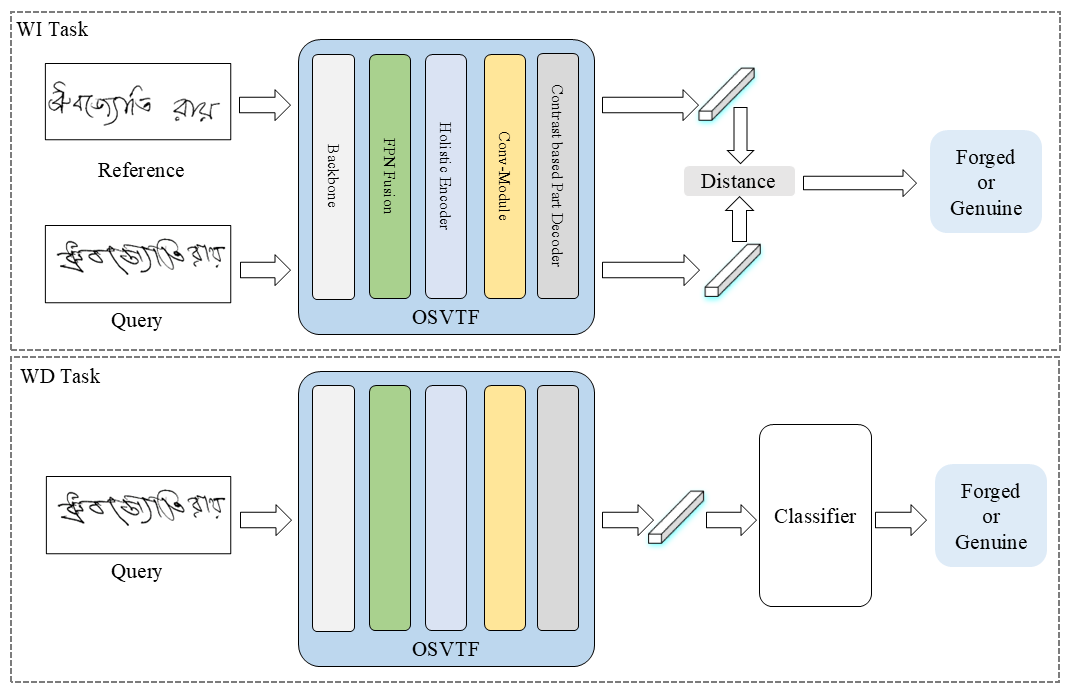
\includegraphics[scale=0.5]{figure/overview.png}
    \end{center}
    \caption{OSVTF overview}
    \label{fig:overview}
\end{figure}

The core idea of the siamese network is two sub-networks with shared weights that accept two inputs and output two feature vectors, and subsequently calculate the similarity using a distance function \cite{10}. In the WI and WD tasks of offline handwritten signature verification, a pair of images of the inputreference and query signatures are input, so the overall architecture is referred to TransOSV \cite{41}, based on which the backbone and FPN Fusion modules are added, and the Encoder, Conv-Module, and Decoder sections are subjected to a The Encoder, Conv-Module and Decoder parts are optimized and adjusted in a series of ways, which are more conducive to the change and learning of the features of each part, and the experimental part is needed to confirm that these modules can improve the model's ability of judging forged signatures and generalization ability in different scenarios.

In the overall research plan and experiments, the two general directions of WI and WD are still adopted to evaluate the performance and quality of the model as a whole, based on which the multi-channel feature maps of CNN and the attention mechanism of Transformer will be visualized, and we need to pay attention to whether these modules are able to better grasp some of the important feature information of the image in the image feature learning. In addition, there are many ways of fusion of multi-scale features, such as Mask R-CNN \cite{13} takes the feature pyramid network style (FPN-Style) \cite{23}, this kind of fusion includes, but is not limited to, mean accumulation, direct summation, and splicing, so the follow-up will be to train the model of these fusion methods with the control variables in order to get the best performance of fusion of multi-scale feature maps way. In addition, the previous twin network approach is to calculate the similarity based on the distance function in order to complete the related tasks, whether this approach can still be effective after the addition of multi-scale fusion features requires some verification, this work will refer to the traditional image classification task of the CNN processing classification approach, the addition of a global average pooling layer as a classifier to classify the features label prediction, in order to determine whether it would be outperform the previous distance similarity judgment.

In summary, this work will be divided into three parts of the research phase: 1. Initially, the OSVTF model architecture will be trained in the model cycle to verify whether the optimized and adjusted scheme of multi-scale features and models can be improved on the original architecture; 2. For the multi-scale fusion method of the FPN Fusion module, a small fine-tuning training will be taken on the basis of the first phase of the control variable method for the model, and the best multi-scale feature fusion method will be selected. The best multi-scale feature fusion method; 3. For the WD task, a global average pooling classifier is added in the final classifier stage, which is compared with the previous method of distance similarity prediction for offline handwritten signature verification, so as to judge the advantages and disadvantages of the two classifiers, and a better classifier is adopted for experiments in the WD task to verify whether it works.

\chapter{Figures and Tables}
In Biometrics technology, handwritten signatures are more important personal identity verification features, and the core challenge of its verification algorithms or models lies in the high intraclass variation of signatures (natural variations of signatures of the same person) and the low interclass variation (similarity between forged signatures and real signatures), and the models and algorithms will be evaluated based on these two directions. The handwritten signature verification task, on the other hand, is categorized into offline and online verification depending on how the image data is processed. In this work, we focus on the offline handwritten signature verification task with static images, which is different from online verification in that the user's signature is dynamically accepted on the digitizing device, i.e., the handwriting data is changing in real time, and all the information from the beginning to the end of the process of writing will be collected; and the offline verification is completely through the static image data in order to carry out the user's verification, which does not set any limitations on the digitizing device, and it only needs to be done through the This method does not set any limitations on the digitizing device, and only requires the author to write on a form, thus greatly reducing the workload in the data collection process.

The image data collected by offline handwritten signature needs to be pre-processed to a certain extent for model or algorithm validation, and good data pre-processing techniques will to a certain extent improve the system validation accuracy. In order to improve the quality of signature images, scholars have adopted the image processing of converting RGB images to GRAY single-channel images and smoothing pixels to remove noise [37]. This processing can well reduce the unnecessary features of handwritten signature images collected on white paper, such as the value of some channel pixel points in the RGB three-channel image is 255, while the value of pixel points with handwritten handwriting is often very small. However, this processing method has the defect that the value of the pixel points in the part with handwriting features is very small while the value of the pixel points in the other blank parts is very large, so the subsequent scholars processed these images with black and white inversion, and it was verified that this processing method can get a better verification accuracy rate [11].

In the early stage of offline signature verification in the 1990s-2000s period, scholars based on geometric features to distinguish the authenticity of the signature image sample pairs [29], by manually extracting the image aspect ratio, stroke length and other global features and inflection points, curvature, and other local features for matching recognition. This approach laid the initial feature extraction template for offline signature verification, where similarity calculation is performed after manual feature extraction. In 1996, Lee et al. proposed template matching for offline signature verification, which aligns the signature trajectories by dynamic time regularization (DTW) to determine whether the signature is forged or not [20]. With the development of statistical theory, two schools of work emerged in the 2000s-2010s period: feature engineering dominated by a series of feature design and classifier design. In 2011, Vargas et al. mentioned for the first time the introduction of feature engineering into feature extraction for offline signature verification by combining texture engineering (LBP, HOG) with structural features (gradient direction distribution). These feature engineering will lead to a drastic increase in the number of signature image features, thus requiring scholars to start adopting machine learning approaches in order to act as classifiers, e.g., Edson et al. proposed an offline signature verification system in 2005 using Hidden Markov Models [17], where the HMM model focuses on modeling the variation of the allowable changes in signatures, i.e., treating each pixel of the image as a word vector, in order to better capture the relationship between the strokes relationships; Malik et al. in 2013 used SVM as a classifier to accomplish handwritten signature verification with higher dimensional feature counts, SVM is one of the most commonly used classifiers for binary classification tasks among academics, and it can also deal with high feature dimensions, so most of the follow-ups have taken SVM in the classifier stage. Even though traditional machine learning methods have improved the performance of early signature verification systems, they still have the defect of relying greatly on manual feature extraction, and manually designing a large number of feature extraction steps will lead to too large a difference in the individual feature parts, which cannot ensure that the merged feature vectors can be statistically significant, and manually designing the features is difficult to capture complex patterns, such as pen pressure and local texture. Moreover, the models trained by this method have insufficient generalization ability, are poorly adapted to cross-dataset and cross-linguistic scenarios, and are extremely costly in terms of computational time [26].

With the development of computer hardware, offline handwritten signatures are gradually transitioning to deep learning. The early stage of deep learning was a development process dominated by convolutional neural networks, and in 2012 Krizhevsky A. et al. proposed AlexNet [19] to win the ImageNet competition's image classification task far ahead of the second-place participant using traditional machine learning algorithms, which made deep learning represented by convolutional neural networks gradually become the mainstream method for image tasks. Subsequently, academics introduced a deeper convolutional neural network, VGG [32], which is an architecture that adds more convolutional layers on top of AlexNet to extract more channels of feature maps. However, this computation of stacked convolutional layers makes the feature map size smaller while leading to the loss of features at each stage, in order to solve this problem, in 2016 K. He et al. proposed ResNet with residual connectivity [14]. A residual connection is added between the convolutional layers of each size feature map to accumulate the feature maps from the original input model layer to the output feature maps. This way in supervised learning convolutional neural network, after weight sharing convolutional kernel operation, can somewhat compensate for the original image feature information, and this residual connection becomes the mainstream way of retaining local features in subsequent deep models. The high-quality performance of convolutional neural networks on image classification tasks has led to offline handwritten signature verification to start resorting to convolutional neural networks in order to replace the earlier step of manually designing features. In 2017, L. G. Hafemann et al. used convolutional neural networks to extract signature image features for the first time for verification [11], adopting the convolutional partial operation to output feature maps as signature image features, and designing two fully-connected layers in the output stage to share the signature image features to output the author ID and signature category. This approach combines both WI and WD tasks, satisfies both outputs and is shown to significantly improve the accuracy of offline signature verification. This approach and its reliance on model training skills, the training process and its difficulty in achieving parameter convergence results, but also provides ideas for subsequent handwritten signature verification tasks using deep learning methods. In 2017, Y. Hafemann et al. proposed that using pre-trained CNNs (e.g., VGG) to extract global and local features of signature images and feeding the features into SVMs for classification can significantly improve generalization across datasets [11] with end-to-end optimization. Similarly M. Diaz et al. in 2019 trained CNNs via migration learning combined with SVM as a joint classifier to achieve low error rates on the GPDS dataset [33]. This CNN+SVM approach successfully reduces the error rate of the signature verification task model to a level unmatched by traditional machine learning, which are followed by this deep learning model as a feature extractor and SVM as a joint classifier in order to perform signature verification. And according to the image size of the dataset, S. Dey et al. proposed SigNet [30] in 2020, which fuses multi-scale CNN features with SVM, adopting different scale feature maps outputted from multiple convolutional layers in CNN as signature image features, and optimizing classification boundaries by combining with SVM, and experiments have proved that the multi-scale features will greatly improve the robustness of the overall model, and have a very good model across datasets. The experiments proved that multi-scale features will greatly improve the robustness of the overall model and have very good model performance across data sets. However, CNN has difficulty in capturing the global contextual information of signature images, such as the long-distance dependence between strokes, in the learning ability of signature image features.

With the development of the natural language processing field of deep learning, A. Vaswani et al. proposed the Transformer with Encoder-Decoder architecture based on the attention mechanism in 2017 [34], the attention mechanism can have the ability of global feature awareness for word vectors, which can better capture the contextual information in machine translation tasks with variable sentence lengths. This kind of machine translation task reflects its excellent global generalization ability, and the excellent global context-awareness ability of the architecture is reflected in the translation task across multiple different languages. In view of Transformer's global feature-awareness capability, A. Dosovitskiy et al. first used Transformer's attention mechanism for image classification tasks in 2021, proposing Vision Transformer (ViT) [4] without convolutional operations, which chunks flattens and maps the input image as word vectors to input into Transformer Encoder for attention feature computation, and finally MLP is performed to generate image category probabilities using the feature vectors output from Encoder. This way of image feature processing method that maps the image element as token after mapping, got the recognition accuracy ahead of CNN on Transformer architecture, and reflected the powerful global generalization ability of Transformer on validation and test set, so all kinds of tasks in the field of image gradually began to take the attention mechanism for secondary processing of image features. In 2022, X. Wang et al. for the first time, ViT for offline signature verification, to solve the above CNN is difficult to capture the global context information of the signature image, the use of self-attention mechanism to model the global structure of the signature, to improve the differentiation of complex forged signatures [36], in the GPDS-960 and CEDAR [28] datasets compared to the same period of time the model's Equal Error Rate decreased by 12\%. In 2023 Y. He et al. also proposed TransOSV [38] based on ViT, which is an architecture that provides an end-to-end Transformer-based offline signature verification system that combines both global semantic information and local discrepancy information, and more efficiently utilizes Transformer for local and global feature modeling. It introduces a multi-layer feature combination mechanism that splices features from different modules into the final signature representation to achieve multi-angle detection of forged signatures; meanwhile, Focal Contrast Loss is designed based on the Focal Loss [10] of the comparison task and the handling of the sample imbalance Double-Margin Loss [24] to solve the above problems while Enhance the learning of HARD SAMPLES in the public dataset of offline signature task, and also incorporate the comparison learning of different module features. And unlike the previous twin networks for offline signature verification, the part decoder is proposed, which locates and focuses on the sensitive parts of forged signatures by comparing the token-level ATTENTION of REFERENCE and QUERY, and introduces the weight of the ATTENTION mechanism into the part features of the decoder, which enhances the model's perception of the part location of forged signatures. However, TransOSV still has defects, it adopts a multi-layer feature combination mechanism to detect signature image pairs of features from different perspectives, but it does not have a strong generalization ability in the case of different signature image scales, and the decoder part does not have a good abstract expression ability for token-level features.

In summary, this work will add backbone to extract multi-scale feature maps on the basis of TransOSV architecture, and adopt FPN Fusion to fuse multi-scale features in order to enhance the learning of multi-scale features by the model architecture. At the same time, in order to better abstract expression of multi-scale fusion features in the subsequent modules, the Conv-Module is designed with downsampling structure, and the input mapping as well as the multi-head adjustment of cross-attention are added in the part decoder, which enhances the model's ability of abstract expression of image features, and is able to strengthen the attention to the forged signatures after the learning of global contextual attention features in the Encoder localized sensitive regions. On the WD task, a global average pooling layer [21] will be provided for signature category prediction as per the traditional image classification task due to the adoption of a large number of convolutional output feature maps and a multi-layer feature combination mechanism.


% \section{Figures}
% \begin{figure}[H]
% 	\centering
% 	\begin{minipage}{.48\textwidth}
% 		\centering

% 		\begin{tikzpicture}[scale=1.8]
% 		\begin{axis}[tiny]
% 		\addplot+ [scatter] {cos(deg(x))};
% 		\end{axis}
% 		\end{tikzpicture}

% 		\captionof{figure}{A figure.}
% 		\label{fig:test1}
% 	\end{minipage}%
% 	\begin{minipage}{.48\textwidth}
% 		\centering
		
% 		\begin{tikzpicture}[scale=1.8]
% 		\begin{axis}[tiny]
% 		\addplot+ [scatter,
% 		mark repeat=3,mark phase=2]
% 		{sin(deg(x))};
% 		\end{axis}
% 		\end{tikzpicture}
			
% 		\captionof{figure}{Another figure.}
% 		\label{fig:test2}
% 	\end{minipage}
% \end{figure}


% Fig. \ref{fig:test1} and Fig. \ref{fig:test2} represent two figures. In what follows, we draw an automaton using \LaTeX. All the sizes of elements in a drawing can be controlled.


% \begin{figure}[htbp]
% \begin{center}
% 	\begin{tikzpicture}
% 				[->,>=stealth',shorten >=1pt,auto,node distance=3.5cm,
% 				semithick,scale=.6,bend angle=45]
% 				%%%右箭头,箭头样式,自动适应,node默认间距,线条默认半粗,比例,默认弯角
% 				\tikzstyle{every state}=[fill=blue!30,draw=blue!75,text=black,minimum size=6mm,scale=1.5]
% 				%默认state样式为蓝色(0-100)填充,蓝色线条,黑色文本,最小size,比例
% 				%画出所有node
% 				\node[state,scale=0.4](0)                       {};
% 				%大括号内是node中的内容,(0)为该node的代号
% 				\node[state,scale=0.4](1) [below left of=0]     {};
% 				%[]内为(1)在(0)的左下位置,默认间距
% 				\node[state,scale=0.4](2) [below right of=0]    {};
% 				\node[draw=white]at(90:2)                       {}
% 				%一个不画出的node,由角坐标给出位置,注意这里还没有分号
% 				edge[<->](0);%其后可以直接定义edge,以分号结束指令
				
				
% 				%在node之间添加连线.第一个中括号中内容是连线的性质(颜色、弯曲方向和角度)
% 				%第二个括号中的内容是每条连线所附带的字母与连线的相对位置。有right\left\below\above可选
% 				\path 
% 				(0)edge [red,bend angle=30,bend right]node[above]{$\alpha$}      (1) %0到1
% 				(1)edge [bend angle=30,bend right]    node[right]{$\beta$}       (0)  
% 				(1)edge                               node[below]{$\lambda$}     (2)
% 				(2)edge [red,bend angle=30,bend right]node[above]{$\mu$}         (0)
% 				;%完整指令后以分号结束
% 			\end{tikzpicture}
% \end{center}
% \caption{This is an automaton.}
%     \label{fig:my_label}
% \end{figure}



% \begin{figure}[htbp]
% \centering
% \begin{tikzpicture}[>=stealth]
% 	\node (state0) [draw=blue,fill=blue!20,xshift=2cm] {$(\{0,2\},\{0,2\})$};
% 	\node (state1) [draw=blue,fill=blue!20,left=1cm of state0.center,yshift=-1.5cm] {$(\{2\},\{0,2\})$};
%     \node (state2) [draw=blue,fill=blue!20,right=1cm of state0.center,yshift=-1.5cm] {$(\{1,3\},\{0,2\})$};
%     \node (state3) [draw=blue,fill=blue!20,below=1.3cm of state1.center] {$(\{1,3\},\{1,3\})$};
%     \node (state4) [draw=blue,fill=blue!20,below=1.3cm of state2.center] {$(\{2\},\{2\})$};
%     \node (state5) [draw=blue,fill=blue!20,below=1.3cm of state3.center] {$(\{2\},\{1,3\})$};
%     \node (state6) [draw=blue,fill=blue!20,below=1.3cm of state4.center] {$(\{1,3\},\{2\})$};
%     \draw[->,line width=1pt]  (2,1) -- (state0.north);
%     \draw [->,line width=1pt,dashed] (state0) to node [right] {\footnotesize$a_{i}$} (state2);
% 	\draw [->,line width=1pt,dashed] (state1) to node [above] {\footnotesize$a_{i}$} (state2);
%     \draw [->,line width=1pt,dashed] (state2.south west) to [in=340,out=200] node [above] {\footnotesize$c_{i}$} (state1.south east);
%     \draw [->,line width=1pt,dashed] (state3.south) to node [left] {\footnotesize$c_{i}$} (state5.north);
% 	\draw [->,line width=1pt,dashed] (state5.east) to [in=330,out=10] node [left] {\footnotesize$a_{i}$} (state3.south east);
%     \draw [->,line width=1pt,dashed] (state4.south) to  node [left] {\footnotesize$a_{i}$} (state6.north);
%     \draw [->,line width=1pt,dashed] (state6.east) to [in=330,out=30] node [left] {\footnotesize$c_{i}$} (state4.south east);
%     \draw [->,line width=1pt] (state1) to node [left] {\footnotesize$a$} (state3);
%     \draw [->,line width=1pt] (state3) to node [below] {\footnotesize$c$} (state4);
%     \draw [->,line width=1pt] (state4.north west) to node [above] {\footnotesize$a$} (state3.north east);
%     \draw [->,line width=1pt] (state0.west) to [in=180,out=150] node [left] {\footnotesize$a$} (state3.west);
% \end{tikzpicture}
% \caption{Indicator automaton and verifier of the NFA in Fig. \ref{fig:my_label}}\label{indicator-NFA}
% \end{figure}

% \section{An example of table}
% The table title is at the top of the table.

% \begin{table}[htbp]	
% 	\centering
% 	\caption{A table.}
% 	\begin{tabular}[l]{@{}lcccccc}		
% 		\toprule		
% 		Class$^{\rm a}$ & $\gamma_1$ & $\gamma_2$$^{\rm b}$& $\langle \gamma \rangle$& $G$ & $|{ f}|$ & $\theta _{c}$ \\		
% 		\midrule	
% 		BL Lacs &5 & 36 & 7 & $-4.0$ & $1.0\times 10^{-2}$ & 10$^\circ$ \\		
% 		FSRQs & 5 & 40 & 11 & $-2.3$ & $0.5\times 10^{-2}$ & 14$^\circ$ \\		
% 		\bottomrule		
% 	\end{tabular}
% 	\label{tab:t1}
% \end{table}

% \begin{table}[htbp]  
% \caption{Another table.}  
% \begin{center}  
% \begin{tabu} to 0.8\textwidth{X[c]|X[3,b]|X[2,l]|X[c]|X[3,m]|X[1,c]}  
% %0.8\textwidth   为设置表格宽度  
% %X[c]      表示这一列居中,所占比例为1,相当于X[1,c]  
% %X[3,c]   表示这一列居中,所占比例为3,这列的宽度是X[c]列的3倍  
% \hline  
% $i$  &$x_i$              &$n_i$      &$i$    &$x_i$               &$n_i$\\  
% \hline  
% 1    &0.5$\sim$0.64       &1           &8    &1.48$\sim$1.62      &53\\  
% 2    &0.64$\sim$0.78      &2           &9    &1.62$\sim$1.76      &25\\  
% 3    &0.78$\sim$0.92      &9           &10   &1.76$\sim$1.90      &19\\  
% 4    &0.92$\sim$1.06      &26          &11   &1.90$\sim$2.04      &16\\  
% 5    &1.06$\sim$1.20      &37          &12   &2.04$\sim$2.18      &3\\  
% 6    &1.20$\sim$1.34      &53          &13   &2.18$\sim$2.38      &1\\  
% 7    &1.34$\sim$1.48      &56          &     &                    & \\  
% \hline  
% \end{tabu}  
% \end{center}  
% \end{table}

\chapter{Research Method}
\section{Overview}
In this work, we will define the label categories forged as 1 $(y=1)$ and genuine as 0 $(y=0)$ for handwritten signatures, and the input reference signature image is defined as $R \in \mathbb{R}^{H\times W\times 1}$ and the query signature image is defined as $Q \in \mathbb{R}^{H\times W\times 1}$.

\begin{figure}[htbp]
  \begin{center}
      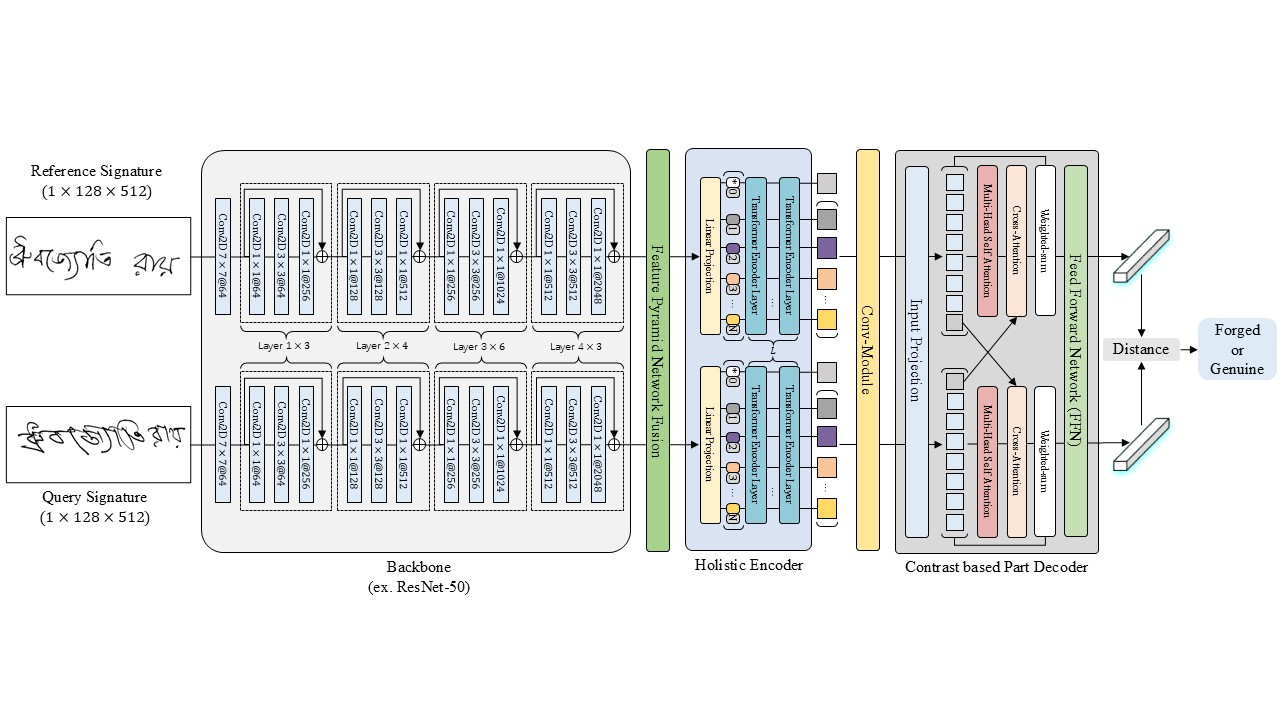
\includegraphics[scale=0.46]{figure/osvtf.jpg}
  \end{center}
  \caption{OSVTF structure Detail}
  \label{fig:osvtf}
\end{figure}

The architecture of the proposed Offline Signature Verification TransFormer (OSVTF) model for multi-scale feature fusion is shown in Fig. \ref{fig:osvtf}, which consists of five parts, namely, Backbone ($\mathcal{B}$), FPN Fusion ($\mathcal{F}$), Holistic Encoder ($\mathcal{H}$), and Conv-Module ($\mathcal{C}$), Contrast based Part Decoder ($\mathcal{P}$) five parts. In the model we will input a pair of signature image samples $\mathbf{I}_r$ and $\mathbf{I}_q$, the initial input image goes through Backbone with shared weights (ResNet-50 \cite{14} is used as an example in Fig. \ref{fig:osvtf}) to get the multi-scale feature map set $\mathcal{B}(\mathbf{I}_r),\mathcal{B}(\mathbf{I}_q)$, and then the different scale feature maps are fused through FPN Fusion module, and the output of multi-scale fusion feature maps $\mathbf{F}_r^\mathcal{F},\mathbf{F}_q^\mathcal{F}$. Then it enters the Holistic Encoder with shared weights to get the holistic flat features $f_r^\mathcal{H},f_q^\mathcal{H}$ and patch embeddings $\boldsymbol{x}_r^\mathcal{H}=[x_r^{\mathcal{H}_1 }, \cdots, x_r^{\mathcal{H}_N} ]$ and $\boldsymbol{x}_q^\mathcal{H} = [ x_q^{\mathcal{H}_1}, \cdots, x_q^{\mathcal{H}_N} ]$. To further integrate the feature maps, the above patch embeddings are reshaped to a 2D shape, and its outputs $\mathbf{F}_r^\mathcal{C}, \mathbf{F}_q^\mathcal{C}$ are obtained after the Convolutional Module (Conv-Module) with shared weights, and they will go directly to the Contrast based Part Decoder to obtain the cross-attention contrast part flat features $f_r^\mathcal{P},f_q^\mathcal{P}$. In the final prediction stage, Global Average Pooling (GAP) operation is performed on $\mathbf{F}_r^\mathcal{F},\mathbf{F}_q^\mathcal{F}$ and $\mathbf{F}_r^\mathcal{C},\mathbf{F}_q^\mathcal{C}$ to obtain the multiscale fusion flat features $f_r^\mathcal{F},f_q^\mathcal{F}$ and convolution flat features $f_r^\mathcal{C},f_q^\mathcal{C}$. The total feature vector $f_r=[f_r^\mathcal{F},f_r^\mathcal{H},f_r^\mathcal{C},f_r^\mathcal{P} ]$ and $f_q=[f_q^\mathcal{F},f_q^\mathcal{H},f_q^\mathcal{C},f_q^\mathcal{P} ]$ of the OSVTF are obtained by splicing all the flat features, and the judgment of whether $\mathbf{I}_q$ is forged or not will be made based on $f_r$ and $f_q$. Next, Backbone, FPN Fusion, Holistic Encoder, Conv-Module and Contrast based Part Decoder structures will be analyzed in depth.

\section{Backbone}

In the Backbone section an architecture of CNN will be adopted that discards Average Global Pooling and Fully Connected Layers in the output section.Most of the CNN architecture consists of a convolutional layer in the input section and four defined convolutional layers, as shown in Fig. 3 for example in ResNet-50 \cite{14}, where each layer consists of a number of bottleneck blocks. A single bottleneck block consists of two convolutional 2D layers with convolutional kernels of ($1\times 1 \to 3\times 3 \to 1\times 1$), and this arrangement mainly has the following purposes: 1. Reduce the feature dimensions to achieve the purpose of improving the computational efficiency; 2. The intermediate $3\times 3$ convolution extracts the local spatial features such as strokes, edges, etc., in the lower dimensional space has the ability to maintain the sensory field while reducing the redundancy, and this reduces the number of channels before expanding to the input, and then the number of channels is expanded to the input, and the number of channels is reduced. This first reduces the number of expression channels and then expands to the input expression channels to find better feature learning parameters in the bottomleneck, which has a better feature abstraction and expression ability; 3. In the actual operation, it can be paired with the identity skip connection to quickly propagate the gradient to avoid gradient disappearance, and at the same time, such a design makes the number of intermediate parameters and the burden of computation greatly reduced, and it can stack more layers. At the same time, this design can greatly reduce the number of intermediate parameters and computational burden, and can stack more layers, such as ResNet-101, to promote the training of deeper networks; 4. This modular design has the advantage of easy fine-tuning of the convolutional parameters, and the number of intermediate channels can be adjusted according to the environment, so as to control the balance of performance and efficiency. In addition, ResNet series network introduces residual connection, which solves the problem of missing features after deep convolutional operation of the image. Residual connection is introduced in each bottomleneck block, which accumulates the feature map of the input part with the output of the bottomleneck, which can reduce the problem of feature loss after a certain number of convolutional layer operations to a certain extent.

Assume that the input feature map $ \mathbf{I} \in \mathbb{ R }^{ H\times W\times C } $ of the convolutional layer, the output feature map $\boldsymbol{z} \in \mathbb{ R }^{ H'\times W'\times C' }$, the convolutional kernel size of the convolutional 2D layer $K\times K$ (the convolutional kernel weight $ \tilde{\mathbf{W}} \in \mathbb{ R }^{ K\times K\times C\times C' } $, the padding $\tilde{P}$, the step size $\tilde{S}$, and the bias term $\tilde{b}$. For the $c'$-th output channel of the feature map, the pixel point with spatial location $(i,j)$ is calculated as eq. \ref{eq1}.

\begin{equation}
\label{eq1}
  \boldsymbol{z}(i, j, c') = \sum^{C'}_{c=1} \sum^K_{u=1} \sum^K_{v=1} = \tilde{\mathbf{W}}_{u, v, c, c'} \cdot \mathbf{I}(i\cdot \tilde{S}+u-\tilde{P}, j\cdot \tilde{S}+v - \tilde{P}, c) + \tilde{\mathbf{b}}_{c'}
\end{equation}

In addition, in each bottleneck block, except for the last $1\times 1$ convolutional 2D layer which is followed only by the BatchNorm (BN) \cite{16} operation, each convolutional 2D layer will be followed immediately by the BN and ReLU activation function \cite{29} operation (Conv2D$\to$BN$\to$ReLU), and the spatial location $(i,j,c')$ after the BN and ReLU activation function is the pixel point values are as eq. \ref{eq2}.

\begin{equation}
\label{eq2}
  \hat{\boldsymbol{z}}(i, j, c') = \max \left( 0, \gamma_c \frac{\boldsymbol{z}(c', i, j) - \mu'_c}{\sqrt{\sigma^2_{c'}+\epsilon}}+\beta_{c'} \right)
\end{equation}

Where $\mu,\sigma^2$ are the mean and variance of the feature statistics of the $c'$ channel plane in the batch multi-channel feature maps output from the convolutional 2D layer, and $\gamma, \beta$ are the learnable scaling and translation parameters. This shows that the idea of the BN operation is to normalize a certain batch of data, which has the effect of improving the convergence speed when training the model parameters. In each bottomleneck block operation, a cumulative residual operation is performed on the feature maps after three convolutional 2D operations, i.e., the feature maps input to the bottomleneck block are added to the feature maps output from the three convolutional 2D operations, which are then passed to the next bottomleneck block. At the same time, each layer of the backbone operation will be followed by a downsampling operation as a way to reduce the redundant features on the multi-channel feature map, which will be taken as Max Pooling 2D in order to equate the downsampling operation \cite{14}. The above residual linking approach can ensure that the feature map retains certain original image features after the convolution operation, so the ResNet family of networks is most suitable as the backbone of the depth model to extract the image multi-channel feature map.

The backbone is taken mainly to extract the image multi-scale feature maps, so the different scale feature maps of each layer except the input convolutional layer are included in the final output as eq. \ref{eq3}.

\begin{equation}
\label{eq3}
  \mathcal{B}(\mathbf{I}) = \{ \mathbf{F}^{\mathcal{B}(1)}, \mathbf{F}^{\mathcal{B}(2)}, \mathbf{F}^{\mathcal{B}(3)}, \mathbf{F}^{\mathcal{B}(4)} \}
\end{equation}

where the multi-channel feature map $\mathbf{F}^\mathcal{B}(i) \in \mathbb{R}^{\frac{H}{2^{i+1}} \times \frac{W}{2^{i+1}} \times \frac{C}{2^{i-1}}},(i=1,2,3,4)$ for each scale, H,W,C denote the width, height and the number of channels of the output feature maps of layer 1, and $C=256$ when the backbone is ResNet-50), and each layer of the feature map has a twofold relationship between the channels and dimensions.

\section{FPN Fusion}

In order to be able to effectively utilize the multi-scale feature maps extracted by backbone, the Feature Pyramid Network Fusion (FPN Fusion) module is used in order to fuse feature maps at different scales, which adopts the model architecture of FPN-Style \cite{23}, as shown in Figure \ref{fig:fpn}.

\begin{figure}[htbp]
  \begin{center}
      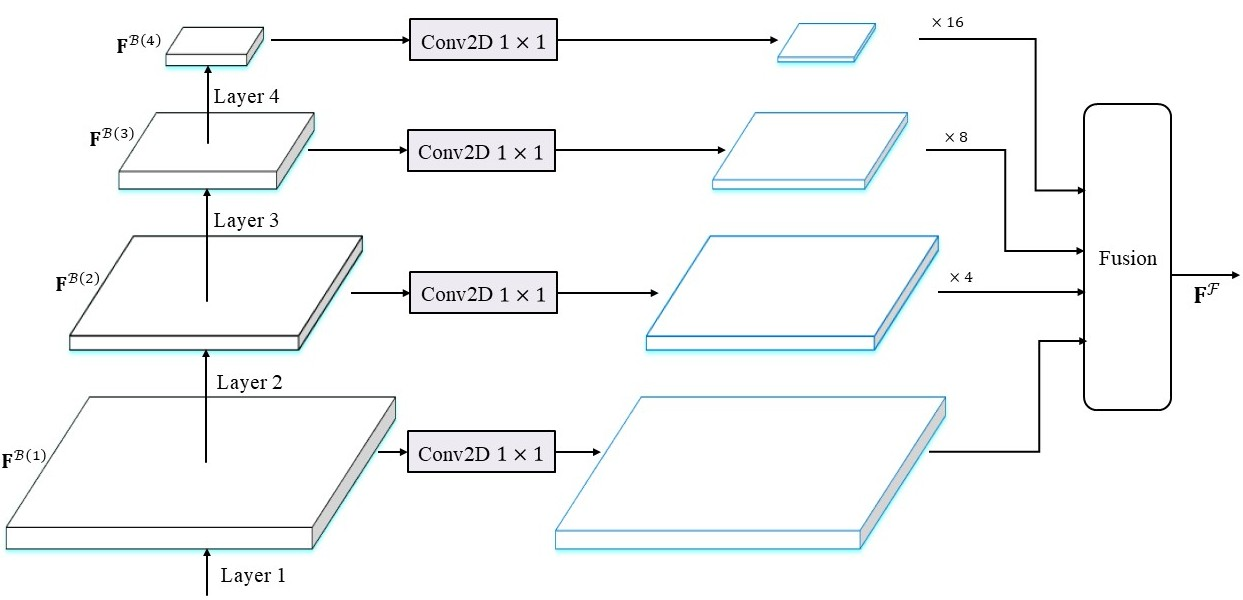
\includegraphics[scale=0.45]{figure/fpn.jpg}
  \end{center}
  \caption{FPN Fusion module structure}
  \label{fig:fpn}
\end{figure}

Where the bottom-up process is the process of backbone inference to obtain different scales of feature maps. In bottom-down, for each layer of feature maps, a convolutional 2D layer with a convolutional kernel of $1\times 1$ will be taken for mapping, which maps the feature maps with different number of channels at each scale to the same feature dimensions, and achieves the operation of dimensionality reduction to a certain extent, so as to accelerate the speed of model inference. At the same time, $\mathbf{F}^{\mathcal{B}(2)} ,\mathbf{F}^{\mathcal{B}(3)} ,\mathbf{F}^{\mathcal{B}(4)}$ are up-sampled to increase the size to the same size as $\mathbf{F}^{\mathcal{B}(1)}$, and then fused according to the fusion method in order to get the multi-scale fusion feature map. Bilinear interpolation \cite{18} is adopted in the up-sampling process, for the lth layer feature map up-sampling output $\mathbf{F}^{\mathcal{B}(l)}$, the value of spatial location $(i',j',c)$ is calculated as eq. \ref{eq4}.

\begin{equation}
\label{eq4}
  \begin{aligned}
    \mbox{Up}(\mathbf{F}^{\mathcal{B}(l)})(i', j', c) &= (1-\delta_i)(1-\delta_j)\cdot \mathbf{F}^{\mathcal{B}(l)}(i, j, c)\\
    &+\delta_i(1-\delta_j)\cdot \mathbf{F}^{\mathcal{B}(l)}(i+1, j, c) \\
    &+(1-\delta_i)\delta_j\cdot \mathbf{F}^{\mathcal{B}(l)}(i, j+1, c) \\
    &+\delta_i \delta_j \cdot \mathbf{F}^{\mathcal{B}(l)}(i+1, j+1, c)
  \end{aligned}
\end{equation}

where $\delta_i=\frac{i'}{s_i} - \lfloor \frac{i'}{s_i} \rfloor, \delta_j = \frac{j'}{s_j} - \lfloor \frac{j'}{s_j} \rfloor$ denote fractional portions of the value in the direction of the width and the height, $s_i,s_j$ denote the magnification $(s_i = s_j = 2)$, and $\lfloor \cdot \rfloor$ denotes the value of the integer part. This up-sampling method can well preserve the original feature ground structure while introducing a smooth transition as shown in Fig. \ref{fig:bilinear}. 

\begin{figure}[htbp]
  \centering
  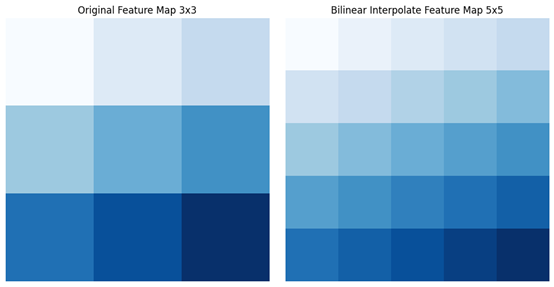
\includegraphics[scale=0.8]{figure/bilinear.png}
  \caption{Bilinear interpolation example}
  \label{fig:bilinear}
\end{figure}

Each up-sampled pixel point will be weighted according to the original feature map pixel points, which not only retains the structural scale of the original feature map, but at the same time makes the transition between pixel points smoother, and to a certain extent, it can reflect the effect of different scales on the image feature points, for example, the features of a certain stroke will be enlarged.

After each scale feature map is sampled on the ground by bilinear interpolation, it will be fused according to three ways: accumulation, weighted average, and channel splicing. The first way is the traditional FPN-Style approach, which directly performs the accumulation operation on the downscaled multi-scale feature maps directly, similar to the residual link mentioned above. The design idea of the second way is to be able to ensure that the signature images of different scenarios can have a certain learning ability, by setting the proportion of weights to be able to pay more attention to the features of a certain scale, and the default is to take all equal weights. The third way is to splice in the channel dimension, followed by a convolutional kernel $1\times 1$ convolutional 2D operation, this method can maximize the retention of all scales of features, but may lead to the model computational overhead is too large, resulting in slower convergence of the model.

After fusing the multi-scale feature map, it will finally go through a convolutional 2D layer with a convolutional kernel $3\times 3$ to smooth out the checkerboard artifacts brought about by the up-sampling process, and finally output the multi-scale fused feature map $\mathbf{F}^\mathcal{F} = \mathcal{F}(\mathcal{B}(\mathbf{I})) \in \mathbb{R}^{\frac{H}{4}\times \frac{W}{4}\times C}$.

\section{Holistic Encoder}

\begin{figure}[H]
  \begin{center}
      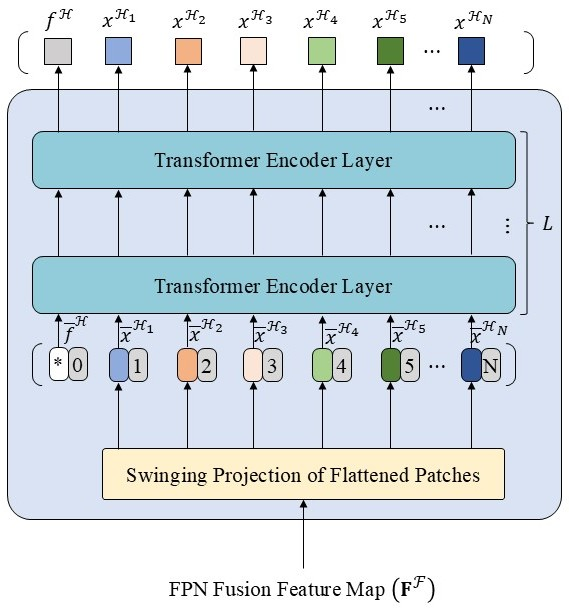
\includegraphics[scale=0.6]{figure/encoder.jpg}
  \end{center}
  \caption{Holistic Encoder structure}
  \label{fig:encoder}
\end{figure}

The Holistic Encoder is designed with reference to Vision Transformer (ViT) \cite{4} The architecture is shown in Fig. 6. swing embeddings \cite{24} are adopted in the input stage instead of the previous chunking operation, where chunking and mapping are performed on the input multiscale fusion feature maps according to the set window size $P\times P$ and step size S , the patch embeddings are obtained and then flattened to be used as feature vectors $[\overline{x}^{\mathcal{H}_1},\overline{x}^{\mathcal{H}_2},\cdots ,\overline{x}^{\mathcal{H}_N}] \in \mathbb{R}^{N\times D}$, where D denotes the number of mapped feature dimensions, and the vector length, $N$, is computed as eq. \ref{eq5}.


\begin{equation}
\label{eq5}
  N=\lfloor \frac{H/4-P+S}{S}\rfloor \times \lfloor \frac{W/4-P+S}{S}\rfloor
\end{equation}

Splicing a learnable weight $\overline{f}^{\mathcal{H}}\in \mathbb{R}^D$ defined as a class token in swing embeddings, i.e., the feature vector of the input Transformer Encoder Layer is $\overline{\boldsymbol{x}}^\mathcal{H}=[\overline{f}^\mathcal{H},\overline{x}^{\mathcal{H}_1},\overline{x}^{\mathcal{H}_2},\cdots ,\overline{x}^{\mathcal{H}_N} ] \in \mathbb{R}^{(N+1)\times D}$. Due to the flattening operation performed on the feature map, positional embeddings \cite{36} need to be accumulated on the feature vectors as a way to make the feature vectors contain information about their positions on the multiscale fused feature map.

After swing embeddings, the feature vector $\overline{\boldsymbol{x}}^\mathcal{H}$ enters the Transformer Encoder Layer for attention feature computation. Where Transformer Encoder Layer is formed by $L$ stacks as shown in Fig. \ref{fig:mhsa}.

\begin{figure}[H]
  \begin{center}
      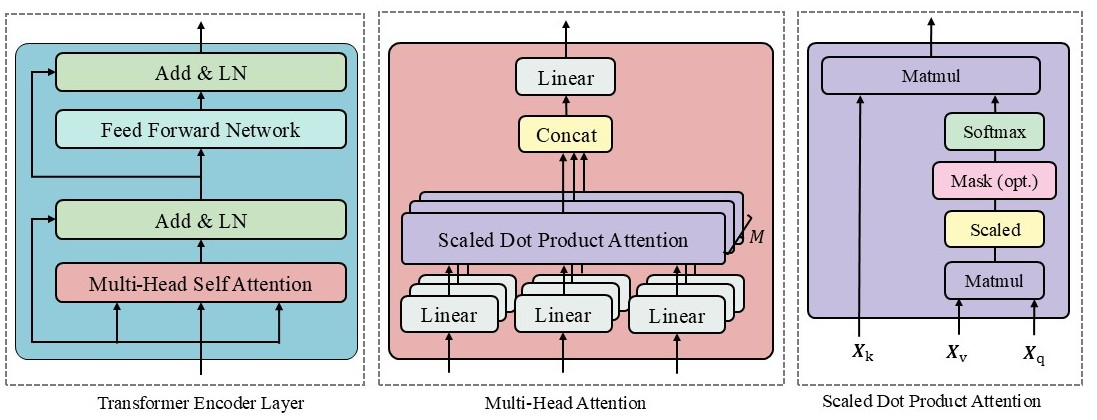
\includegraphics[scale=0.55]{figure/mhsa.jpg}
  \end{center}
  \caption{Transformer Encoder Layer structure}
  \label{fig:mhsa}
\end{figure}

Each Transformer Encoder Layer consists of a Multi-Head Self Attention $\to$ Add \& LN and Feed Forward Network $\to$ Add \& LN, where Add \& LN denotes residual linking and LayerNormalization (LN) \cite{1}. The input feature vectors first enter Multi-Head Self Attention (MHSA) in order to perform the computation of the attention mechanism, which is essentially Multi-Head Attention (MHA) except that the sources before the mapping of $\boldsymbol{X}_\text{q} \in \mathbb{R}^{N\times d_q}$ and $\boldsymbol{X}_\text{k}, \boldsymbol{X}_\text{v} \in \mathbb{R}^{N\times d_k }$ in the operations are The same, i.e., the input feature vectors will be simultaneously entered into the linear mapping layer of each head for dimensionality reduction, thus generating the query vector $\boldsymbol{X}_\text{q}$, the key vector $\boldsymbol{X}_\text{k}$, the value vector $X_v$, and $d_q = d_k$. where the attention mechanism is divided into multiple head computations in order to conserve the computational resources, and the feature vectors will be entered into the three linear layers of the $M$ heads in order to be dimensionality reduced for mapping, thus achieving the attention computation in parallel, and the final splice and linear layer mapping will input vectors with the same feature dimensions, so the output vector shape of MHSA is the same as the input vector shape. The attention feature vectors of each head in MHSA are computed by taking scaled dot product attention \cite{36} with the following eq. \ref{eq6}.

\begin{equation}
\label{eq6}
  \text{Attn}(\boldsymbol{X}_\text{v}, \boldsymbol{X}_\text{k}, \boldsymbol{X}_\text{v}) = \text{Softmax} \left( \frac{\boldsymbol{X}_\text{q}\boldsymbol{X}_\text{k}^\mathrm{T}}{\sqrt{d_k}} \right)\cdot \boldsymbol{X}_\text{v}
\end{equation}

In this case, there is a soft query relationship between $\boldsymbol{X}_\text{q}, \boldsymbol{X}_\text{k}$ and $\boldsymbol{X}_\text{v}$. Instead of selecting a specific key-value pair for each query, all key-values are weighted and averaged, and the weights are computed by the similarity between $\boldsymbol{X}_\text{q}$ and $\boldsymbol{X}_\text{k}$. each feature token of $\boldsymbol{X}_\text{q}$ establishes a relevance distribution, i.e., a Softmax \cite{37} of attention weights, based on which the values of $\boldsymbol{X}_\text{v}$ are weighted and fused. The advantage of this mechanism is that it can focus on multiple relevant tokens at the same time, which enables the model to more fully model the contextual information, for example, the $(i, j)$ position of attention weight indicates the weight of $i$-th position of $\boldsymbol{X}_\text{q}$ on the $j$-th position of $\boldsymbol{X}_\text{k}$, the larger the value of this weight, the stronger the contextual relationship of the query at the $i$-th position to the key at $j$-th position, and conversely the smaller the value, the relationship is very small. According to this attention weight, multiplying $\boldsymbol{X}_\text{v}$ again will further amplify the features in the place where the attention weight of its own vector is high, and the attention information will be included between tokens, so as to achieve that each token owns its own global information, and can more effectively utilize the important features and ignore the useless features, and will more effectively pay attention to the part of the brush strokes in the image of the handwritten signature, ignoring the blank part. The resulting MHSA output of a single Transformer Encoder Layer is as eq. \ref{eq7}.

\begin{equation}
\label{eq7}
\text{MHSA}(\overline{\boldsymbol{x}}^\mathcal{H},\mathbf{T},\mathbf{L}) =
\begin{bmatrix}
  \text{Attn}(\overline{\boldsymbol{x}}^\mathcal{H} \mathbf{T}_{1,1},\overline{\boldsymbol{x}}^\mathcal{H} \mathbf{T}_{1,2},\overline{\boldsymbol{x}}^\mathcal{H} \mathbf{T}_{1,3}) \\
  \text{Attn}(\overline{\boldsymbol{x}}^\mathcal{H} \mathbf{T}_{2,1},\overline{\boldsymbol{x}}^\mathcal{H} \mathbf{T}_{2,2},\overline{\boldsymbol{x}}^\mathcal{H} \mathbf{T}_{2,3}) \\
  \cdots \\
  \text{Attn}(\overline{\boldsymbol{x}}^\mathcal{H} \mathbf{T}_{m,1},\overline{\boldsymbol{x}}^\mathcal{H} \mathbf{T}_{m,2},\overline{\boldsymbol{x}}^\mathcal{H} \mathbf{T}_{m,3}) \\
\end{bmatrix}^{\mathrm{T}}
\cdot \mathbf{L} 
\end{equation}

where $\mathbf{T}_l \in \mathbb{R}^{M\times 3\times d_k\times d_k' }$ denotes the linear mapping layer weights in the input phase of the MHSA, $\mathbf{L} \in \mathbb{R}^{d_k\times d_k' }$ denotes the weights of the final linear mapping layer in the MHSA, and $d_k'$ denotes the number of feature dimensions of each head $\boldsymbol{X}_\text{q}, \boldsymbol{X}_\text{k}$ and $\boldsymbol{X}_\text{v}$, and thus must satisfy $d_k=M\times d_k'$.

Matrix multiplication with larger dimensions is performed in the MHSA section, and in order to reduce the risk of gradient explosion or vanishing, and also to reduce the missing information of the original feature vectors, a residual link and an LN layer follow immediately after the MHSA.The main role of the LN layer is to normalize the feature vectors at each position, thus speeding up the convergence of the model as well as improving the model stability. Unlike the mean and variance of the BN, the mean and variance of the LN are derived from the current feature dimensions on which they are calculated as eq. \ref{eq8}.

\begin{equation}
\label{eq8}
\begin{aligned}
  \mu &= \frac{1}{d_k}\sum^{d_k}_d \text{MHSA}(\overline{\boldsymbol{x}}^\mathcal{H}, \mathbf{T}, \mathbf{L})_d \\
  \sigma^2 &= \frac{1}{d_k}\sum^{d_k}_d \left( \text{MHSA}(\overline{\boldsymbol{x}}^\mathcal{H}, \mathbf{T}, \mathbf{L})_d - \mu \right)^2
\end{aligned}
\end{equation}

where $\text{MHSA}(\overline{\boldsymbol{x}}^\mathcal{H},\mathbf{T},\mathbf{L})_d$ denotes the dth feature dimension of the MHSA output feature vector. The subsequent normalization operation is the same as in the BN layer, and the entire MHSA$\to$Add \& LN output is computed as eq. \ref{eq9}.

\begin{equation}
\label{eq9}
  \hat{\text{MHSA}}(\overline{\boldsymbol{x}}^\mathcal{H}, \mathbf{T}, \mathbf{L}) = \gamma \cdot \left( \frac{\text{MHSA}(\overline{\boldsymbol{x}}^\mathcal{H}, \mathbf{T}, \mathbf{L}) - \mu}{\sqrt{\sigma^2+\epsilon}} + \mathcal{E}_{l-1} \right) + \beta
\end{equation}

Where $\mathcal{E}_{l-1}$ denotes the output of the previous Transformer Encoder Layer, if $l=1$, then $\mathcal{E}_{l-1}=\overline{\boldsymbol{x}}^\mathcal{H}$. After the attention computation, Feed Forward Network (FFN) is introduced to enhance the overall model to model the complex patterns \cite{8}, and the whole FFN is computed as eq. \ref{eq10}:

\begin{equation}
\label{eq10}
  \text{FFN}(\hat{\text{MHSA}}(\overline{\boldsymbol{x}}^\mathcal{H}, \mathbf{T}, \mathbf{L})) = \mathcal{G}(\hat{\text{MHSA}}(\overline{\boldsymbol{x}}^\mathcal{H}, \mathbf{T}, \mathbf{L})\mathbf{W}_1 + \mathbf{b}_1)\mathbf{W}_2 + \mathbf{b}_2
\end{equation}

Where $\mathbf{W}_1\in \mathbb{R}^{D\times d_{ff}}, b_1\in \mathbb{R}^{d_{ff}}$ denotes the weight and bias of the first linear layer in the FFN, and $\mathbf{W}_2\in \mathbb{R}^{d_{ff}\times D}, \mathbf{b}_2\in \mathbb{R}^D$ denotes the weight and bias of the second prior layer in the FFN, $\mathcal{G}$ denotes the GeLU function \cite{15}. the GeLU function and the ReLU function act similarly as the activation function that performs the nonlinear transformation. The entire FFN is a nonlinear transformation of the model, which complements the global interaction mechanism of Attention to jointly build a powerful context-aware representation. Subsequently followed by Add \& LN to supplement the feature information and accelerate the model convergence, each subsequent layer of Transformer Encoder Layer is a stacking effect to deepen the Attention weight of the feature vectors, and the output of the whole Holistic Encoder is $\{f^\mathcal{H}, \boldsymbol{x}^\mathcal{H} \} = \mathcal{H}(F^\mathcal{F}),f^H\in \mathbb{R}^D,x^\mathcal{H} \in R^{N\times D}$.

\section{Conv-Module}

The image features are subjected to feature learning by Holistic Encoder capturing the relative position information of the elements in the sequence, but it has the limitation of learning absolute position information. The signature verification task needs to be accurate to the stroke position information (e.g., stroke order, local structural differences), so after this in order to enhance some small portion of the image features, the output $\boldsymbol{x}^\mathcal{H}$ of the patch token of the Holistic Encoder is rearranged, and the flattened token is reconverted into a 2D shape $\mathbf{F}^\mathcal{H} \in \mathbb{R}^{h\times w\times D}$ to perform a convolution operation, where $h = \lfloor \frac{H/4-P+S}{S}\rfloor,w = \lfloor \frac{W/4-P+S}{S}\rfloor $. This module introduces the convolution operation to reprocess the patch features output from the Transformer encoder to enhance the position-awareness. In the Conv-Module architecture, the Conv design of TransOSV \cite{41} is referenced, and the number of output channels of the intermediate convolutional 2D layer is adjusted to increase the downsampling operation according to the style of previous CNNs, as shown in Table \ref{tab:conv}.


\begin{table}[htbp]
\caption{Conv-Module layers information}  
\begin{center}
\begin{tabu} to 0.8\textwidth{X[3, c]X[3, c]X[3, c]}  
%0.8\textwidth   为设置表格宽度  
%X[c]      表示这一列居中,所占比例为1,相当于X[1,c]  
%X[3,c]   表示这一列居中,所占比例为3,这列的宽度是X[c]列的3倍  
\toprule
Layer & Kernel Size & Output feature map\\
\midrule
Conv2D + ReLU & $3\times 3$ & $h\times w\times d_\mathcal{C}$ \\ 
Conv2D + ReLU & $3\times 3$ & $h\times w\times d_\mathcal{C}$ \\ 
Max Pooling 2D & $2\times 2$ & $\frac{h}{2}\times \frac{w}{2}\times d_\mathcal{C}$ \\ 
Conv2D + ReLU & $3\times 3$ & $\frac{h}{2}\times \frac{w}{2}\times \frac{d_\mathcal{C}}{2}$ \\ 
Conv2D + ReLU & $3\times 3$ & $\frac{h}{2}\times \frac{w}{2}\times \frac{d_\mathcal{C}}{2}$ \\ 
Conv2D + ReLU & $3\times 3$ & $\frac{h}{4}\times \frac{w}{4}\times \frac{d_\mathcal{C}}{2}$ \\ 
\bottomrule
\end{tabu}
\end{center}
\label{tab:conv}
\end{table}

Different from the traditional CNN with gradually more channels, the overall downsampling operation thinking is adopted here, and certain downsampling operations are performed on the patch features to abstractly express the local features of the feature map on the basis of integrating the local detail features, with the purpose of enhancing the generalization ability and robustness of the model. This operation is added on the basis of backbone and FPN Fusion to further strengthen the model's ability to perceive the local features of the image, strengthen the focus on the key local regions of the signature, and filter the background interference at the same time. In the Conv-Module module, each Conv2D layer operation is the same as the Conv2D layer operation in backbone, which takes the combination of Conv2D+ReLU, and after two Conv2D+ReLUs a downsampling operation, i.e., Max Pooling 2D operation, will be performed to integrate the feature maps and eliminate the non-important parts of the features to integrate and eliminate non-important parts of the feature map and enhance feature expressiveness.

In the model training process, the output $\mathbf{F}^\mathcal{C} = \mathcal{C}(\mathbf{F}^\mathcal{H} ) \in \mathbb{R}^{h'\times w'\times d_C' }$ of the Conv-Module will undergo a Global Average Pooling (GAP) operation while entering the Contrast based Part Decoder to globally sample the feature maps of the output of the Conv-Module. The feature maps of the Conv-Module are globally sampled to obtain a flat local convolutional feature $f^\mathcal{C}$ to complete the corresponding feature extraction in the training and inference process.

\section{Contrast based Part Decoder}

\begin{figure}[H]
  \centering
      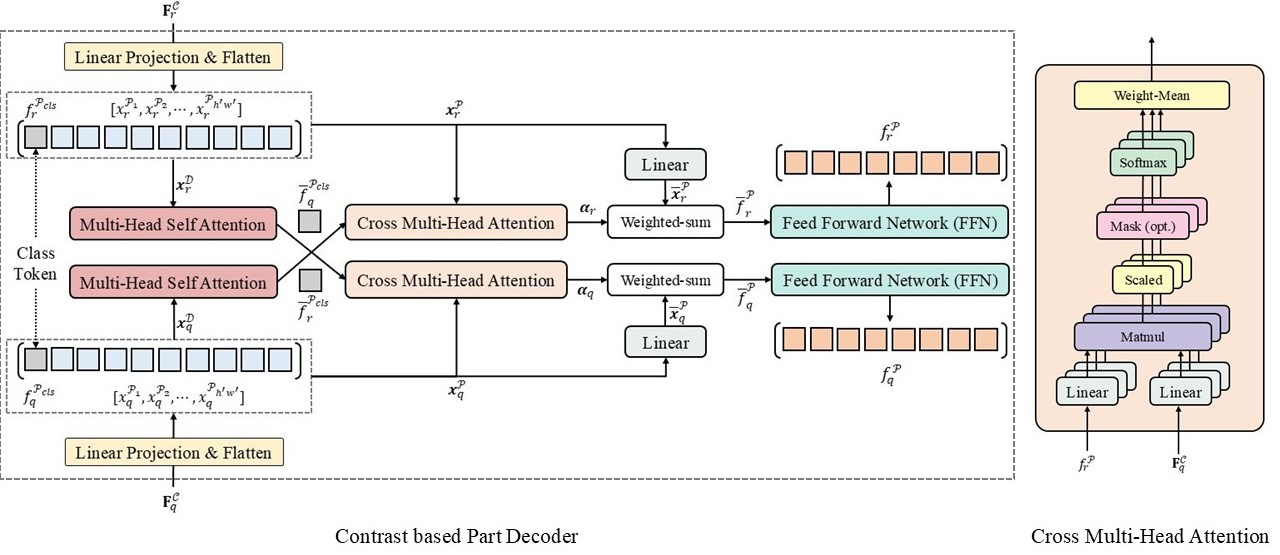
\includegraphics[scale=0.45]{figure/decoder.jpg}
  \caption{Contrast based Part Decoder structure}
  \label{fig:decoder}
\end{figure}

This part is an improvement on TransOSV's Contrast based Part Decoder \cite{41} for parallel computation of Cross-Attention, which references the multi-head attention computation mechanism of MHSA in Holistic Encoder. Similar to the Holistic Encoder part, the feature maps of references and query are mapped to the $d_\mathcal{P}$ feature dimension in the input phase, followed by flattening and addition of a learnable weight $f_r^{\mathcal{P}_{cls}},f_q^{\mathcal{P}_{cls}} \in \mathbb{R}^D$, also defined as a class token, i.e., the input part is obtained as a pair of flattened feature map vectors $\boldsymbol{x}_r^\mathcal{P} = [f_r^{\mathcal{P}_{cls}}, x_r^{\mathcal{P}_1},\cdots ,x_r^{\mathcal{P}_{h' w' }} ]$, $\boldsymbol{x}_q^\mathcal{P}=[f_q^{\mathcal{P}_{cls}},x_q^{\mathcal{P}_1},\cdots,x_q^{\mathcal{P}_{h'w'} } ] \in \mathbb{R}^{h' \times w' \times (D+1)}$. Subsequently, MHSA operations are performed on $\boldsymbol{x}_r^\mathcal{P},\boldsymbol{x}_q^\mathcal{P}$ to take out the class token $\overline{f}_r^{\mathcal{P}_{cls}},\overline{f}_q^{\mathcal{P}_{cls}} \in \mathbb{R}^D$ of their respective output eigenvectors as the query matrix cross-input Cross Multi-Head Attention (CMHA).The structure of CMHA is shown in Figure 8-b shown, differs from MHA in that only the query matrix and key matrix are generated to compute their cross-attention weights $\boldsymbol{\alpha}_r,\boldsymbol{\alpha}_q$, and the final concat is replaced with a weighted average to handle the attention weights of multiple heads. For a single CMHA the output cross-attention weight $\boldsymbol{\alpha}$ is calculated as eq. \ref{eq11}.

\begin{equation}
\label{eq11}
  \boldsymbol{\alpha}= \frac{1}{M}\sum^M_{m=1} \text{Softmax}\left( \frac{\boldsymbol{X}_\text{q}\mathbf{T}^\mathcal{P}_{m, 1}\cdot (\boldsymbol{X}_\text{k}\mathbf{T}^\mathcal{P}_{m, 2})^\mathrm{T} }{\sqrt{d_\mathcal{P}'}} \right)
\end{equation}

where $\boldsymbol{X}_\text{q},\boldsymbol{X}_k$ denote the input query and key vectors, $\mathbf{T}^\mathcal{P} \in \mathbb{R}^{M\times 2\times D\times d_k′}$ denotes the linear mapping layer weights of the input part of the CMHA. The resulting $\boldsymbol{\alpha}_r,\boldsymbol{\alpha}_q$ computation process is as eq. \ref{eq12}.

\begin{equation}
\label{eq12}
\begin{aligned}
  \boldsymbol{\alpha}_r = \frac{1}{M}\sum^M_{m=1} \text{Softmax}\left( \frac{\overline{f}_q^{\mathcal{P}_{cls}}\mathbf{T}^\mathcal{P}_{m, 1}\cdot (\boldsymbol{x}_r^\mathcal{P}\mathbf{T}^\mathcal{P}_{m, 2})^\mathrm{T} }{\sqrt{d_\mathcal{P}'}} \right) \\
  \boldsymbol{\alpha}_q = \frac{1}{M}\sum^M_{m=1} \text{Softmax}\left( \frac{\overline{f}_r^{\mathcal{P}_{cls}}\mathbf{T}^\mathcal{P}_{m, 1}\cdot (\boldsymbol{x}_q^\mathcal{P}\mathbf{T}^\mathcal{P}_{m, 2})^\mathrm{T} }{\sqrt{d_\mathcal{P}'}} \right) \\
\end{aligned}
\end{equation}

Perform a weight-sum operation on the attention weights and the mapped flat feature vector $\overline{\boldsymbol{x}}_r^\mathcal{P},\overline{\boldsymbol{x}}_r^\mathcal{P}\in \mathbb{R}^{h'\times w'\times d_\mathcal{P}}$, and fuse to generate the flat feature $\overline{f}_r^P,\overline{f}_q^P\in \mathbb{R}^{d_P}$ with cross-attention weights. Its after FFN to get the flat feature $\overline{f}_r^\mathcal{P},\overline{f}_q^\mathcal{P}\in \mathbb{R}^{d_P}$ of cross attention of decoder, the whole computation process is as eq. \ref{eq13}.

\begin{equation}
\label{eq13}
  \{f_r^\mathcal{P},f_q^\mathcal{P},\boldsymbol{\alpha}_r,\boldsymbol{\alpha}_q \}=\mathcal{P}(F_r^\mathcal{C},F_q^\mathcal{C} )
\end{equation}

This Contrast based Part Decoder, which is similar to the structure of Transformer Decoder \cite{36}, facilitates the generation of local feature information that distinguishes between genuine and forged signatures, and emphasizes the feature relationship between a pair of data samples, enhancing the model's learning of the features between a pair of data in a sample. During the training process, the output cross-attention weights $\boldsymbol{\alpha}_r,\boldsymbol{\alpha}_q$ are computed with sparsity loss to force the distribution of cross-attention weights to be centralized, avoiding averaging in order to fail to pay attention to the sensitive part of forged signatures.

\section{Loss Funcion}

\subsection{Euclidean Distance}

OSVTF is a model architecture similar to twin networks, this style emphasizes that the model is a two-flow form of shared weights and the overall purpose is to compare the gap between the two, so it will be based on the similarity of the input two features in order to design the loss function. In this work, Euclidean Distance \cite{5} will be taken in order to be used as a similarity calculation for a pair of feature samples, assuming that a pair of features $f_r,f_q$ is input and the formula for calculating the distance between them is as eq. \ref{eq14}.

\begin{equation}
\label{eq14}
  \mathcal{D}(f_r, f_q) = ||f_r - f_q||_2=\sqrt{\sum_{d=1}(f^{(d)}_r - f^{(d)}_q)^2}
\end{equation}

\subsection{Focal Contrast Loss}

In the handwritten signature sample data processing stage, the handwritten signature of the writer will be paired with the pairing operation that will not be repeated between the two, for example, the BHSig-B \cite{3} dataset contains a total of 100 writers' handwritten signature images, in which each writer owns 24 genuine signature images ($y=0$) and 30 forged signature images ($y=1$), the genuine signature images are used as the reference signature, forged signature and real signature together as query signature, which will generate 276 pairs of positive samples and 720 pairs of negative samples. Thus each writer has a total of 996 data sample pairs, in which the ratio between positive and negative sample pairs is not close to 50:50, so the number of positive and negative samples is not balanced and belongs to the category of hard samples \cite{33}. 

The loss function of similarity of comparison samples used for binary classification in earlier algorithms and models is Contrast Loss \cite{10}, which is calculated as eq. \ref{eq15}.

\begin{equation}
\label{eq15}
  \mathcal{L}_c (f_r,f_q ) = (1 - y)\cdot \mathcal{D}(f_r,f_q)^2 + y\cdot \max⁡(m - \mathcal{D}(f_r,f_q),0)^2 
\end{equation}

Where $m$ denotes the boundary value, i.e., the distance that forged samples should be kept at least. For the sample pair of $y=0$, it is directly used as the loss value to make the model parameter learning on the real sample pairs of features more similar; on the contrary $y=1$, if the feature distance between the reference and query is less than $m$, $(m - \mathcal{D}(f_r,f_q ))^2$ is used as the loss value to make the model for the forged signature pairs of features is not less than $m$. However, this kind of loss can't be dynamically emphasized on the hard samples and is prone to model parameter overfitting problems. In order to reduce the risk of overfitting, a boundary value is also introduced for the genuine sample pairs to reduce the unnecessary contraction between the genuine pairs, i.e., the Double-Margin loss \cite{25} is calculated as eq. \ref{eq16}.

\begin{equation}
\label{eq16}
\begin{aligned}
  \mathcal{L}_{dm} (f_r,f_q ) &= (1-y)\cdot \max(\mathcal{D}(f_r,f_q )-n,0)^2 \\
  &+ y\cdot \max⁡(m-\mathcal{D}(f_r,f_q),0)^2
\end{aligned}  
\end{equation}

where the two boundary values m>n, penalize the case where the distance exceeds n for the genuine sample pairs, and promote the case where the distance is greater than m for the forged sample pairs. Although double margin optimizes the problem of easy overfitting by contrast loss to a certain extent, in the case of two pairs of sample data $\{r,q_1 \},\{r,q_2\}$ and $y=1$ In the case, the distance between the two sample pairs is calculated by OSVTF, if $\mathcal{D}(f_r,f_{q_1}) >> \mathcal{D}(f_r,f_{q_2}) > n $, then the loss function should give a greater loss to ${r,q_1}$, but $\mathcal{L}_{dm}$ will treat the two sample pairs equally, and the notion of dynamic weighting is introduced in TransOSV, named Focal Contrast Loss \cite{41}, which is calculated as eq. \ref{eq17}.

\begin{equation}
\label{eq17}
\begin{aligned}
  \mathcal{L}_{fc}(f_r,f_q ) &= (1 - y)\cdot \sigma(\overline{K}(\mathcal{D}(f_r,f_q )-\alpha_1 ))\cdot \max⁡(\mathcal{D}(f_r,f_q)-n,0)^2 \\
  &+ y\cdot \sigma(\overline{V} (\alpha_2 - \mathcal{D}(f_r,f_q))\cdot \max⁡(m - \mathcal{D}(f_r,f_q ))^2 \\
\end{aligned}
\end{equation}

where $\sigma(\boldsymbol{z})=\frac{1}{1+e^{-\boldsymbol{z}}}$, denotes the Sigmoid activation function \cite{26}, which is used to dynamically generate the weights; $\alpha_1,\alpha_2$ are the two margin values; $\overline{K},\overline{V}$ denote the scaling factors, which are used to regulate the scaling factor of the response strength of hard samples. When the label of the sample pair is genuine, if the feature distance is greater than $\alpha_1$, the current weight value is larger; when the label is forged, if the feature distance is smaller than $\alpha_2$, the weight is larger. As a result, $\mathcal{L}_{fc}$ will have the advantages of dynamically adjusting the attention of the training samples, focusing on optimizing the “easily confused” signatures, and improving the generalization ability of the model, and it will be used as one of the main training loss functions of the OSVTF model. According to the flat features extracted from each module, four parts will be taken to calculate the focal contrast loss, and the overall Focal Contrast Loss is calculated as eq. \ref{eq18}.

\begin{equation}
\label{eq18}
  \mathcal{L}_{fc}(f_r,f_q )=
  \begin{bmatrix}
  \lambda_1, \lambda_2, \lambda_3, \lambda_4
  \end{bmatrix} 
  \cdot
  \begin{bmatrix}
  \mathcal{L}_{fc} (f_r^\mathcal{F},f_q^\mathcal{F}) \\
  \mathcal{L}_{fc} (f_r^\mathcal{H},f_q^\mathcal{H}) \\
  \mathcal{L}_{fc} (f_r^\mathcal{C},f_q^\mathcal{C}) \\
  \mathcal{L}_{fc} (f_r^\mathcal{P},f_q^\mathcal{P}) \\
  \end{bmatrix}
\end{equation}

where $\lambda_1,\lambda_2,\lambda_3,\lambda_4$ are training hyperparameters used to assign the weight of each feature.

\newpage
\subsection{Sparsity Loss}

In Contrast based Part Decoder, for the cross attention calculation, the attention weights will be too uniformly distributed, in fact, the model should be enhanced to focus on the most significant local differences in the region, and thus the cross-entropy approach is adopted to generate the entropy constraints of the contrast mask in the hope that the cross-attention weights can be sparsely distributed, thus enhancing the Decoder's local attention accuracy \cite{41}, which is calculated as eq. \ref{eq19}.

\begin{equation}
\label{eq19}
  \mathcal{L}_{spa} (\boldsymbol{\alpha}_r,\boldsymbol{\alpha}_q ) = -\sum_{i=1}^{h'w'} \boldsymbol{\alpha}_q^{(i)}  \log⁡(\boldsymbol{\alpha}_q^{(i)}) 
  - \sum_{i=1}^{h'w'}\boldsymbol{\alpha}_r^{(i)}  \log⁡(\boldsymbol{\alpha}_r^{(i)})
\end{equation}

Since this component is not trained as the main model, ξ is introduced as the hyperparameter of this component to participate in OSVTF training. In summary, the overall loss function of OSVTF is composed as eq. \ref{eq20}.

\begin{equation}
\label{eq20}
  \mathcal{L} = \mathcal{L}_{fc} (f_r,f_q) + \xi\mathcal{L}_{spa} (\boldsymbol{\alpha}_r,\boldsymbol{\alpha}_q)
\end{equation}

\chapter{An example}
\section{Experimental Setup}

In this work, we will build OSVTF based on ViT \cite{4} configuration.The output feature map of The FPN Fusion has the same number of feature dimensions as the number of channels in the first layer of the scaled feature convolution map.The encoder contains 8 Transformer encoder layers ($L\times 8$) and each MHSA in the encoder layer contains 12 heads ($M=12$), 768 features ($D=768$), and a sliding window of size $4\times 4$ steps of $2$ ($P=4,S=2$). In the Conv-Module part, set the number of channels in its intermediate convolutional layer to 512 ($d_\mathcal{C}=512$). In the decoder part, the number of feature dimensions of MHSA and CMHA, and the number of headers are consistent with the parts of encoder, and the number of feature dimensions of weighted-sum's mapping of patch embeddings after CMHA is set to 512
($d_P=512$).

On the loss function, the partial settings $n=0.3,m=0.9,\alpha_1=0.6,\alpha_2=0.8$ and $\overline{K}=\overline{V}=10$ are followed for TransOSV.The hyper-parameters are set to $\lambda_1=0.5,\lambda_2=1.0,\lambda_3=0.5,\lambda_4=2.0,\xi=0.2$.On the optimizer, all experiments are On the optimizer, all experiments are conducted on 2 NVIDIA 3080 GPUs and the total batch size is set to be 16.

\section{Metrics}

In terms of evaluation metrics, unlike conventional binary classification tasks, the offline handwritten signature verification task requires special attention to NEGATIVE samples, and therefore standard metrics in biometric and signature verification tasks \cite{7} are used to evaluate the performance of OSVTF, i.e., False Rejection Rate (FRR), False Acceptance Rate (FAR) and Equal Error Rate (EER). In a conventional binary classification task, the concept of confusion matrix \cite{6} is used to count the number of sample labels and predicted labels in the format of Table \ref{tab:cm}.

\begin{table}[htbp]
\caption{Confusion Matrix}  
\begin{center}
\begin{tabu} to 0.8\textwidth{X[3, c]X[3, c]X[3, c]}  
%0.8\textwidth   为设置表格宽度  
%X[c]      表示这一列居中,所占比例为1,相当于X[1,c]  
%X[3,c]   表示这一列居中,所占比例为3,这列的宽度是X[c]列的3倍  
\toprule
predicted Label / raw label & $\hat{y}=0$ (positive) & $\hat{y}=1$ (negative)\\
\midrule
$y=0$ &  True Positive (TP) & False Negative (FN) \\
$y=1$ & False Positive (FP) & True Negative (TN) \\
\bottomrule
\end{tabu}
\end{center}
\label{tab:cm}
\end{table}

This leads to the following formula for FRR, and FAR:
\begin{equation}
\label{eq21}
\begin{aligned}
	\text{FRR}=\frac{\text{FN}}{\text{FN}+\text{TP}} \\
	\text{FAR}=\frac{\text{FP}}{\text{FP}+\text{TN}}
\end{aligned}
\end{equation}

The EER is calculated using several thresholds and distances for comparison, if the feature distance of the sample pair is greater than the threshold, then its category is forged, otherwise it is genuine. This work will calculate the distance based on the model features of the sample pairs of the batch data during the training process, and based on the distance minima and maxima of the sample pairs in order to set a number of thresholds, so that the FAR and FRR are automatically calculated for the current batch for each threshold value. FAR and FRR are calculated for each threshold and when the difference between FAR and FRR is the smallest, then FRR, FAR for the current threshold are output simultaneously and EER is calculated as follows:

\begin{equation}
\label{eq22}
	\text{EER} = \frac{\text{FRR}+\text{FAR}}{2}	
\end{equation}
	
As a result, the experimental phase will be based on the four evaluation indexes of ACC, FRR, FAR and EER to comprehensively assess the model performance.

\newpage
\section{Dataset}

BHSig-B and BHSig-H. Both datasets are published by Indian Institute of Technology Guwahati (IIT Guwahati) \cite{3} dataset of handwritten signatures in Bengali and Hindi. Where BHSig-B contains Bengali handwritten signatures of 100 writers and BHSig-H contains Hindi handwritten signature images of 160 writers. Each user handwritten signature has signed 24 authentic and 30 forged signatures.
CEDAR. This dataset is an English handwritten signature dataset developed and published by Center of Excellence for Document Analysis and Recognition \cite{30}. It contains 55 handwritten signatures of writers in English. Each user signed 24 authentic and 24 forged signatures by hand.

\section{Results Analysis}

\subsection{Writer-Independent Results}

On the WI task, OSVTF takes the Euclidean distance method to calculate the distance between two features to determine whether the signature is forged or not, in order to evaluate whether OSVTF outperforms the past models in possessing offline handwritten signature verification performance. The initial stage is validated on BHSig-B and BHSig-H, which are consistent with the past algorithms, by dividing the 100 writers of BHSig-B into training and testing sets according to the ratios of 50:50 and 80:20 for 100 writers, and dividing the 160 writers of BHSig-H into training and testing sets according to the ratio of 100:60 for 160 writers. The preliminary experimental results obtained are shown in Table \ref{tab:wi}.

\begin{table}[htbp]
\caption{BHSig-B and BHSig-H dataset WI task performance comparison}  
\begin{center}
\begin{tabu} to 0.8\textwidth{X[3, l]X[2, l]X[2, l]X[2, l]}  
%0.8\textwidth   为设置表格宽度  
%X[c]      表示这一列居中,所占比例为1,相当于X[1,c]  
%X[3,c]   表示这一列居中,所占比例为3,这列的宽度是X[c]列的3倍  
\toprule
Model & FRR & FAR & EER \\
\midrule
BHSig-B \\
\midrule
50/50 \\
SigNet [30] & 13.89 & 13.89 & 13.89 \\
CaP \cite{25} & 3.96 & 3.96 & 3.96 \\
IDN \cite{37}	& 5.24 & 4.12 & - \\
InceptionSVGNet \cite{27} & \bf{2.22} & \bf{3.88} & - \\
TransOSV \cite{41} & 9.90 & 9.90 & 9.90 \\
TransOSV [Ours] & 12.41 & 12.41 & 12.41 \\
OSVTF [Ours] & 10.72 & 10.85 & 10.79 \\
\midrule
80/20			
DeepHsv \cite{21} & 11.92 & 11.92 & 11.92 \\
TransOSV & \bf{3.56} & \bf{3.56} & \bf{3.56} \\
TransOSV [Ours] & 5.11 & 5.11 & 5.11 \\
OSVTF [Ours] & 4.47 & 4.61 & 4.54 \\
\midrule
BHSig-H 100/60 \\
SigNet [30] & 15.36 & 15.36 & 15.36 \\
IDN \cite{37} & 4.93 & 8.99 & - \\
CaP \cite{25} & 5.97 & 5.97 & 5.97 \\
InceptionSVGNet \cite{27} & 3.33 & 6.38 & - \\
TransOSV \cite{41} & \bf{3.24} & \bf{3.24} & \bf{3.24} \\
TransOSV [Ours] & 4.86 & 4.86 & 4.86 \\
OSVTF [Ours] & 3.86 & 3.94 & 3.90 \\
\bottomrule
\end{tabu}
\end{center}
\label{tab:wi}
\end{table}

Among them, in the BHSig-B dataset, 10.79\% EER for OSVTF at 50:50 ratio and 12.41\% EER for reproduced TransOSV, with a difference of about 15.01\%, and 4.54\% EER for OSVTF at 80:20 ratio and 5.11\% EER for reproduced TransOSV, with a difference of about 12.56\%. In the BHSig-H dataset, 4.86\% EER for reproduced TransOSV, 3.90\% EER for OSVTF, a difference of about 24.62\%. The OSVTF performance on the WI task outperforms the TransOSV performance by about 17\%. The performance of OSVTF is slightly inferior to that of TransOSV in the above experimental environments, but the performance of OSVTF compared to TransOSV in the same environments has some improvement, confirming that the multi-scale fusion features of an image have a certain degree of enhancement in the learning ability of the image features on the basis of the combined features. In the BHSig-B 50/50 dataset, OSVTF obtains far less results than CaP, IDN, and InceptionSVGNet, but outperforms the same type of models on the BHSig-B 80/20 and BHSig-H 100/60 datasets, to a certain extent, because these networks are the specialized networks for that scale dataset, and therefore can reflect OSVTF in cross-dataset scenarios is able to adapt to the variations in the images of each dataset to a large extent.

\subsection{Writer-Dependent Results}

On the WD task, in addition to the experiments on the model with the addition of multiscale fusion features, a classifier for the deep learning traditional image classification task (GAP classifier) was added to verify if it is a better fit compared to the SVM's classifier for the model with multiscale fusion features. Therefore, the 80:20 ratio of BHSig-B and BhSig-H were validated and the results are shown in Table \ref{tab:wd}.

\begin{table}[htbp]
\caption{BHSig-B and BHSig-H dataset WD task performance comparison}  
\begin{center}
\begin{tabu} to 0.8\textwidth{X[3, l]X[2, l]X[2, l]X[2, l]}  
%0.8\textwidth   为设置表格宽度  
%X[c]      表示这一列居中,所占比例为1,相当于X[1,c]  
%X[3,c]   表示这一列居中,所占比例为3,这列的宽度是X[c]列的3倍  
\toprule
Model & FRR & FAR & EER \\
\midrule
BHSig-B 80/20 \\
TransOSV [Ours] & 3.78 & 3.78 & 3.78 \\
OSVTF [SVM] & 2.74 & 2.80 & 2.77 \\
OVSTF [GAP] & \bf{2.05} & \bf{2.21} & \bf{2.13} \\
\midrule
BHSig-H 100/60 \\
TransOSV [Ours] & 4.23 & 4.23 & 4.23 \\
OSVTF [SVM] & 3.17 & 3.21 & 3.19 \\
OVSTF [GAP] & \bf{2.67} & \bf{2.69} & \bf{2.68} \\
\bottomrule
\end{tabu}
\end{center}
\label{tab:wd}
\end{table}

Also using SVM as a classifier, in the experimental results on the BHSig-B dataset, OSVTF 2.77\% EER decreased by 36.46\% compared to TransOSV's 3.78\% EER, and in the experimental results on the BHSig-H dataset, OSVTF 3.17\% EER decreased compared to TransOSV's 4.23\% EER by 33.44\%. The OSVTF performance on the WD task outperforms the TransOSV performance by about 34.95\%. On the experimental results of different classifiers, OSVTF 2.13\% EER of BHSig-B taking GAP classifier is better than OSVTF 2.77\% EER taking SVM classifier; OSVTF 2.68\% EER of BHSig-H taking GAP classifier is better than OSVTF 3.19\% EER taking SVM classifier. on the overall WD task, OSVTF of OSVTF also taking SVM classifier outperforms TransOSV by about 34.95\%, and can improve by another 19.03\% when taking GAP classifier. From this, it can be judged that for OSVTF that have adopted multi-scale fusion features, the author classifier that adopts GAP can better handle the above features compared to SVM.


\section{Ablation Experiments}

In the above experimental results, it is shown that OSVTF with the addition of multi-scale fusion features improves the performance on the WI task by about 17\% and on the WD task by about 35\% (and by about 45\% when GAP classification is taken) compared to TransOSV. In this part of the work, ablation experiments will be conducted for the multiscale fusion features, Conv-Module downsampling method, decoder multicast optimization, and sparsity loss in order to verify the performance enhancement of each part for OSVTF, and the obtained WI experimental results are shown in Table \ref{tab:ae}.


\begin{table}[htbp]
\caption{WI task ablation experiments}
\begin{center}
\begin{tabu} to 0.9\textwidth{X[4.5,c]X[2,c]X[2,c]X[2,c]X[2,c]X[9, l]X[9, l]X[8, l]}  
%0.8\textwidth   为设置表格宽度  
%X[c]      表示这一列居中,所占比例为1,相当于X[1,c]  
%X[3,c]   表示这一列居中,所占比例为3,这列的宽度是X[c]列的3倍  
\toprule
Model & $\mathcal{F}$ & $\mathcal{C}$ & $\mathcal{P}$ & $\mathcal{L}_{spa}$ & BHSig-B(80/20) & BHSig-H(100:60) & CEDAR(50:5) \\
\midrule
TransOSV &  &  &  &  & 5.11 & 4.86 & 5.94 \\
Baseline & √ &  &  &  & 4.71 & 4.39 & 5.40 \\
& & √ &  &  & 4.83 & 4.55 & 5.67 \\
&  &  & √ &  & 4.92 & 4.76 & 5.61 \\
& √ & √ & √ &  & 4.64 & 4.21 & 5.21 \\ 
OSVTF & √ & √ & √ & √ & \bf{4.54} & \bf{3.90} & \bf{4.75} \\
\bottomrule
\end{tabu}
\end{center}
\label{tab:ae}
\end{table}

It can be shown that the addition of fusion features of multi-scale feature maps to TransOSV can substantially reduce the model misclassification rate. The Conv-Module with downsampling approach (with simultaneous addition of input mapping in the decoder) enhances the abstract representation of features for more complex modeling operations. In the multi-head optimization of the decoder, multiple perspectives are added to focus on the feature vectors, so the model performance is improved. In the sparsity loss training scheme, the distribution of attention in the decoder is slightly weakened, allowing more attention to be paid to individual local features of the signature image.

In the Conv-Module and decoder part of this work, the mapping structure of dimensionality reduction $\to$ dimensionality enhancement is designed to change the whole Conv-Module from the original change in the number of feature dimensions$ D \to d_\mathcal{C} \to D$ to $D \times d_\mathcal{C} \times \frac{d_\mathcal{C}}{2}$. In order to comply with this change a "dimensionality enhancement" linear mapping layer is introduced at the Encoder input stage. In order to comply with this change, a "dimension-up" linear mapping layer is introduced at the Encoder input stage. In order to verify the feasibility of the "dimensionality reduction→dimensionality enhancement" mapping structure, a large learning rate and 20 training cycles are set in the experiments on the BHSig-B 50/50 dataset, and the changes in the loss function and evaluation indexes before optimization are shown in Fig. 9, and the changes in the loss function and evaluation indexes after optimization are shown in Figs. \ref{fig:bfloss} and \ref{fig:afloss}.

\begin{figure}[H]
	\centering
	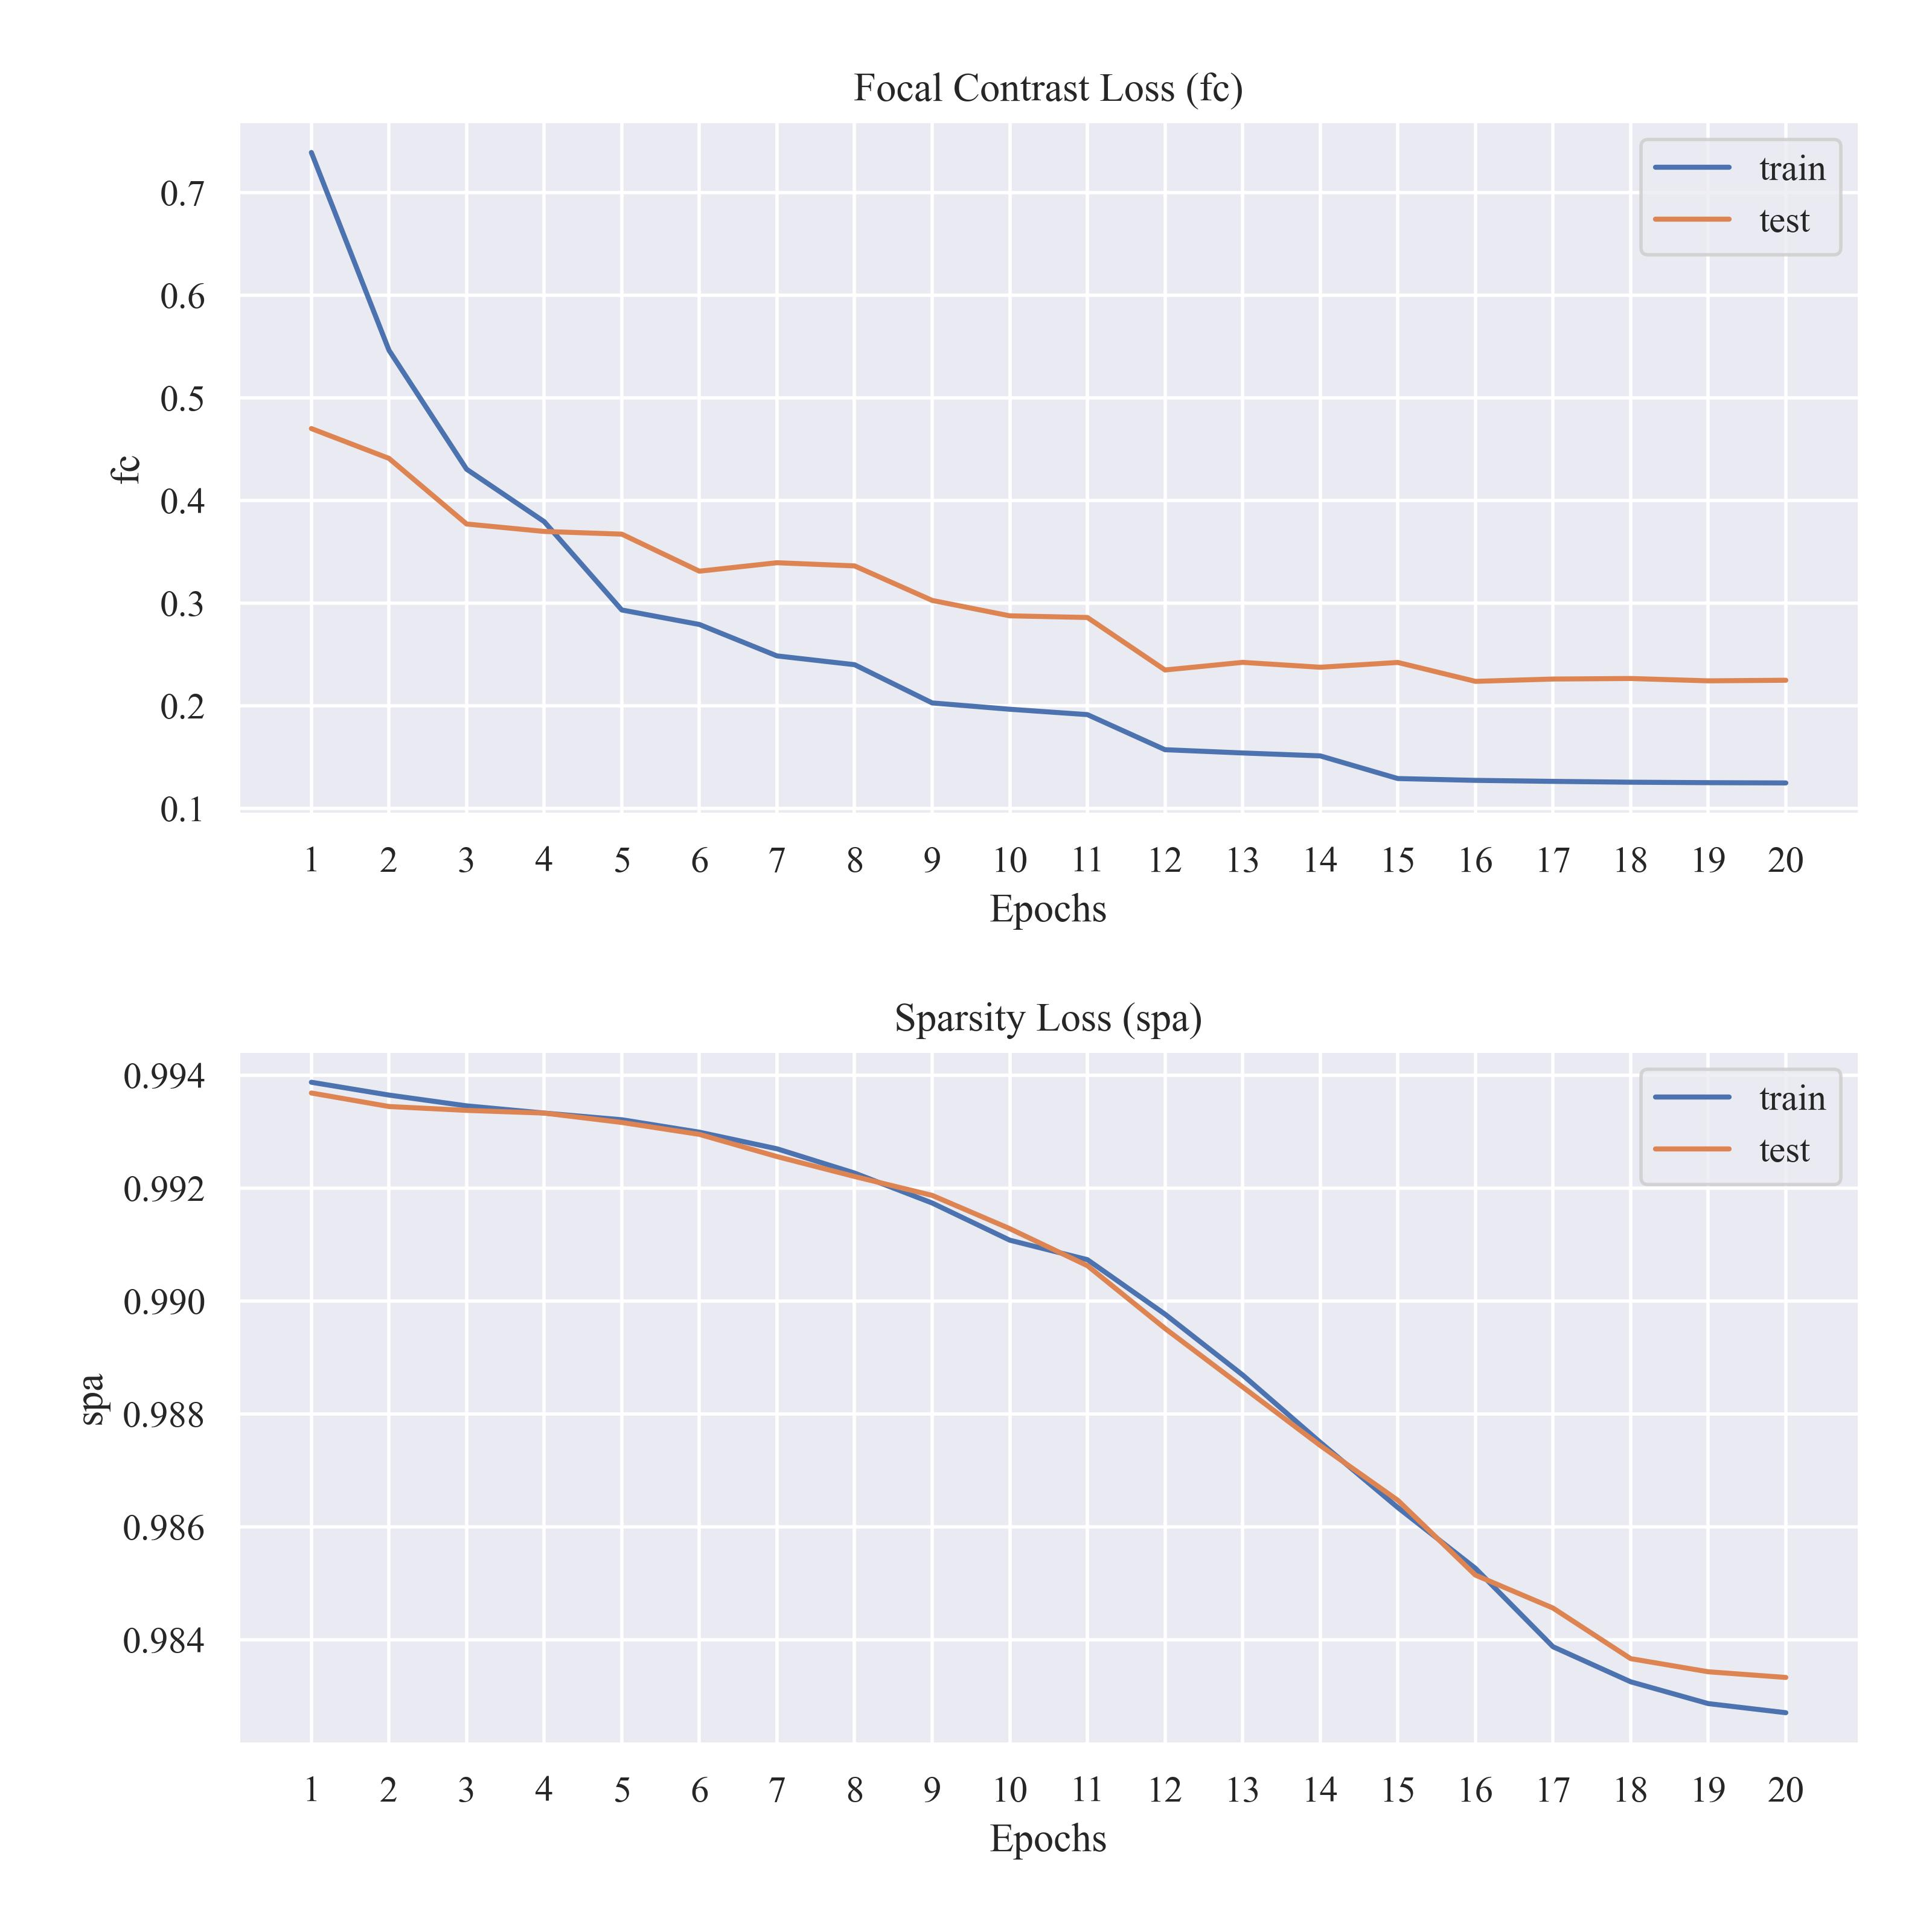
\includegraphics[scale=0.35]{figure/bfloss.jpg}
	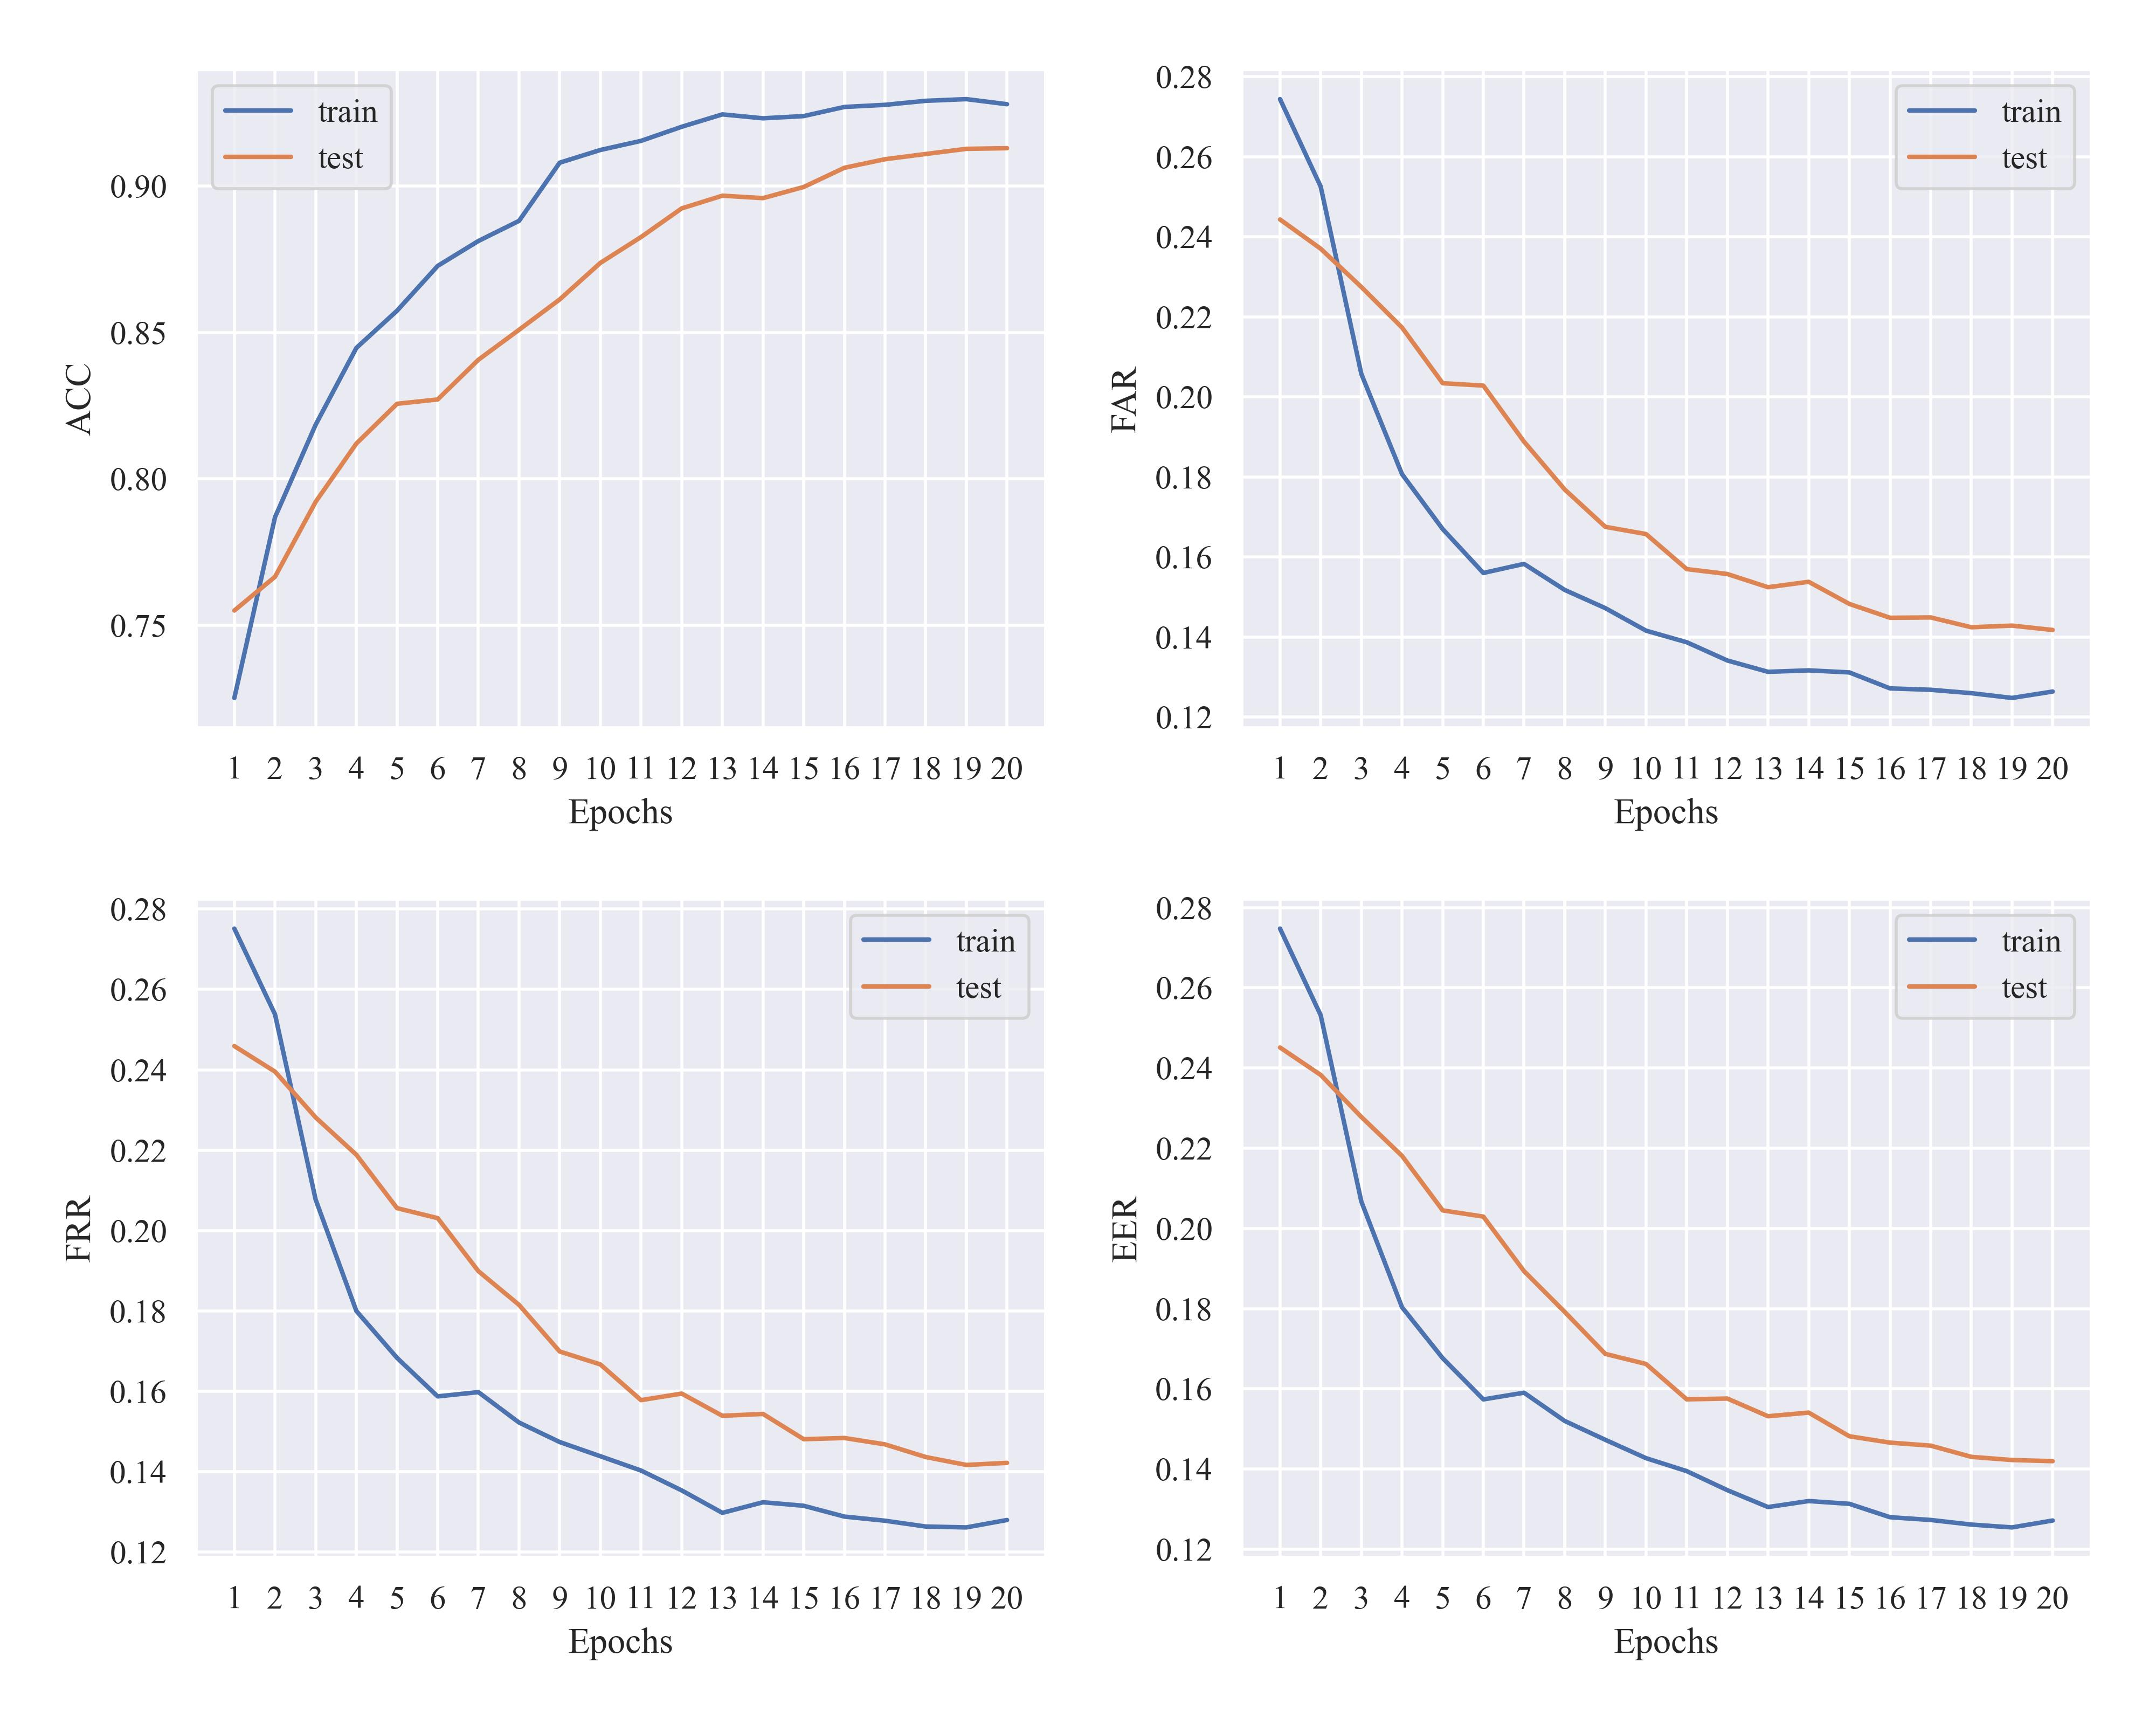
\includegraphics[scale=0.34]{figure/bfmetrics.jpg}
	\caption{Previous Conv-Module loss and metrics diversification}
	\label{fig:bfloss}
  \end{figure}
  
\begin{figure}[H]
\centering
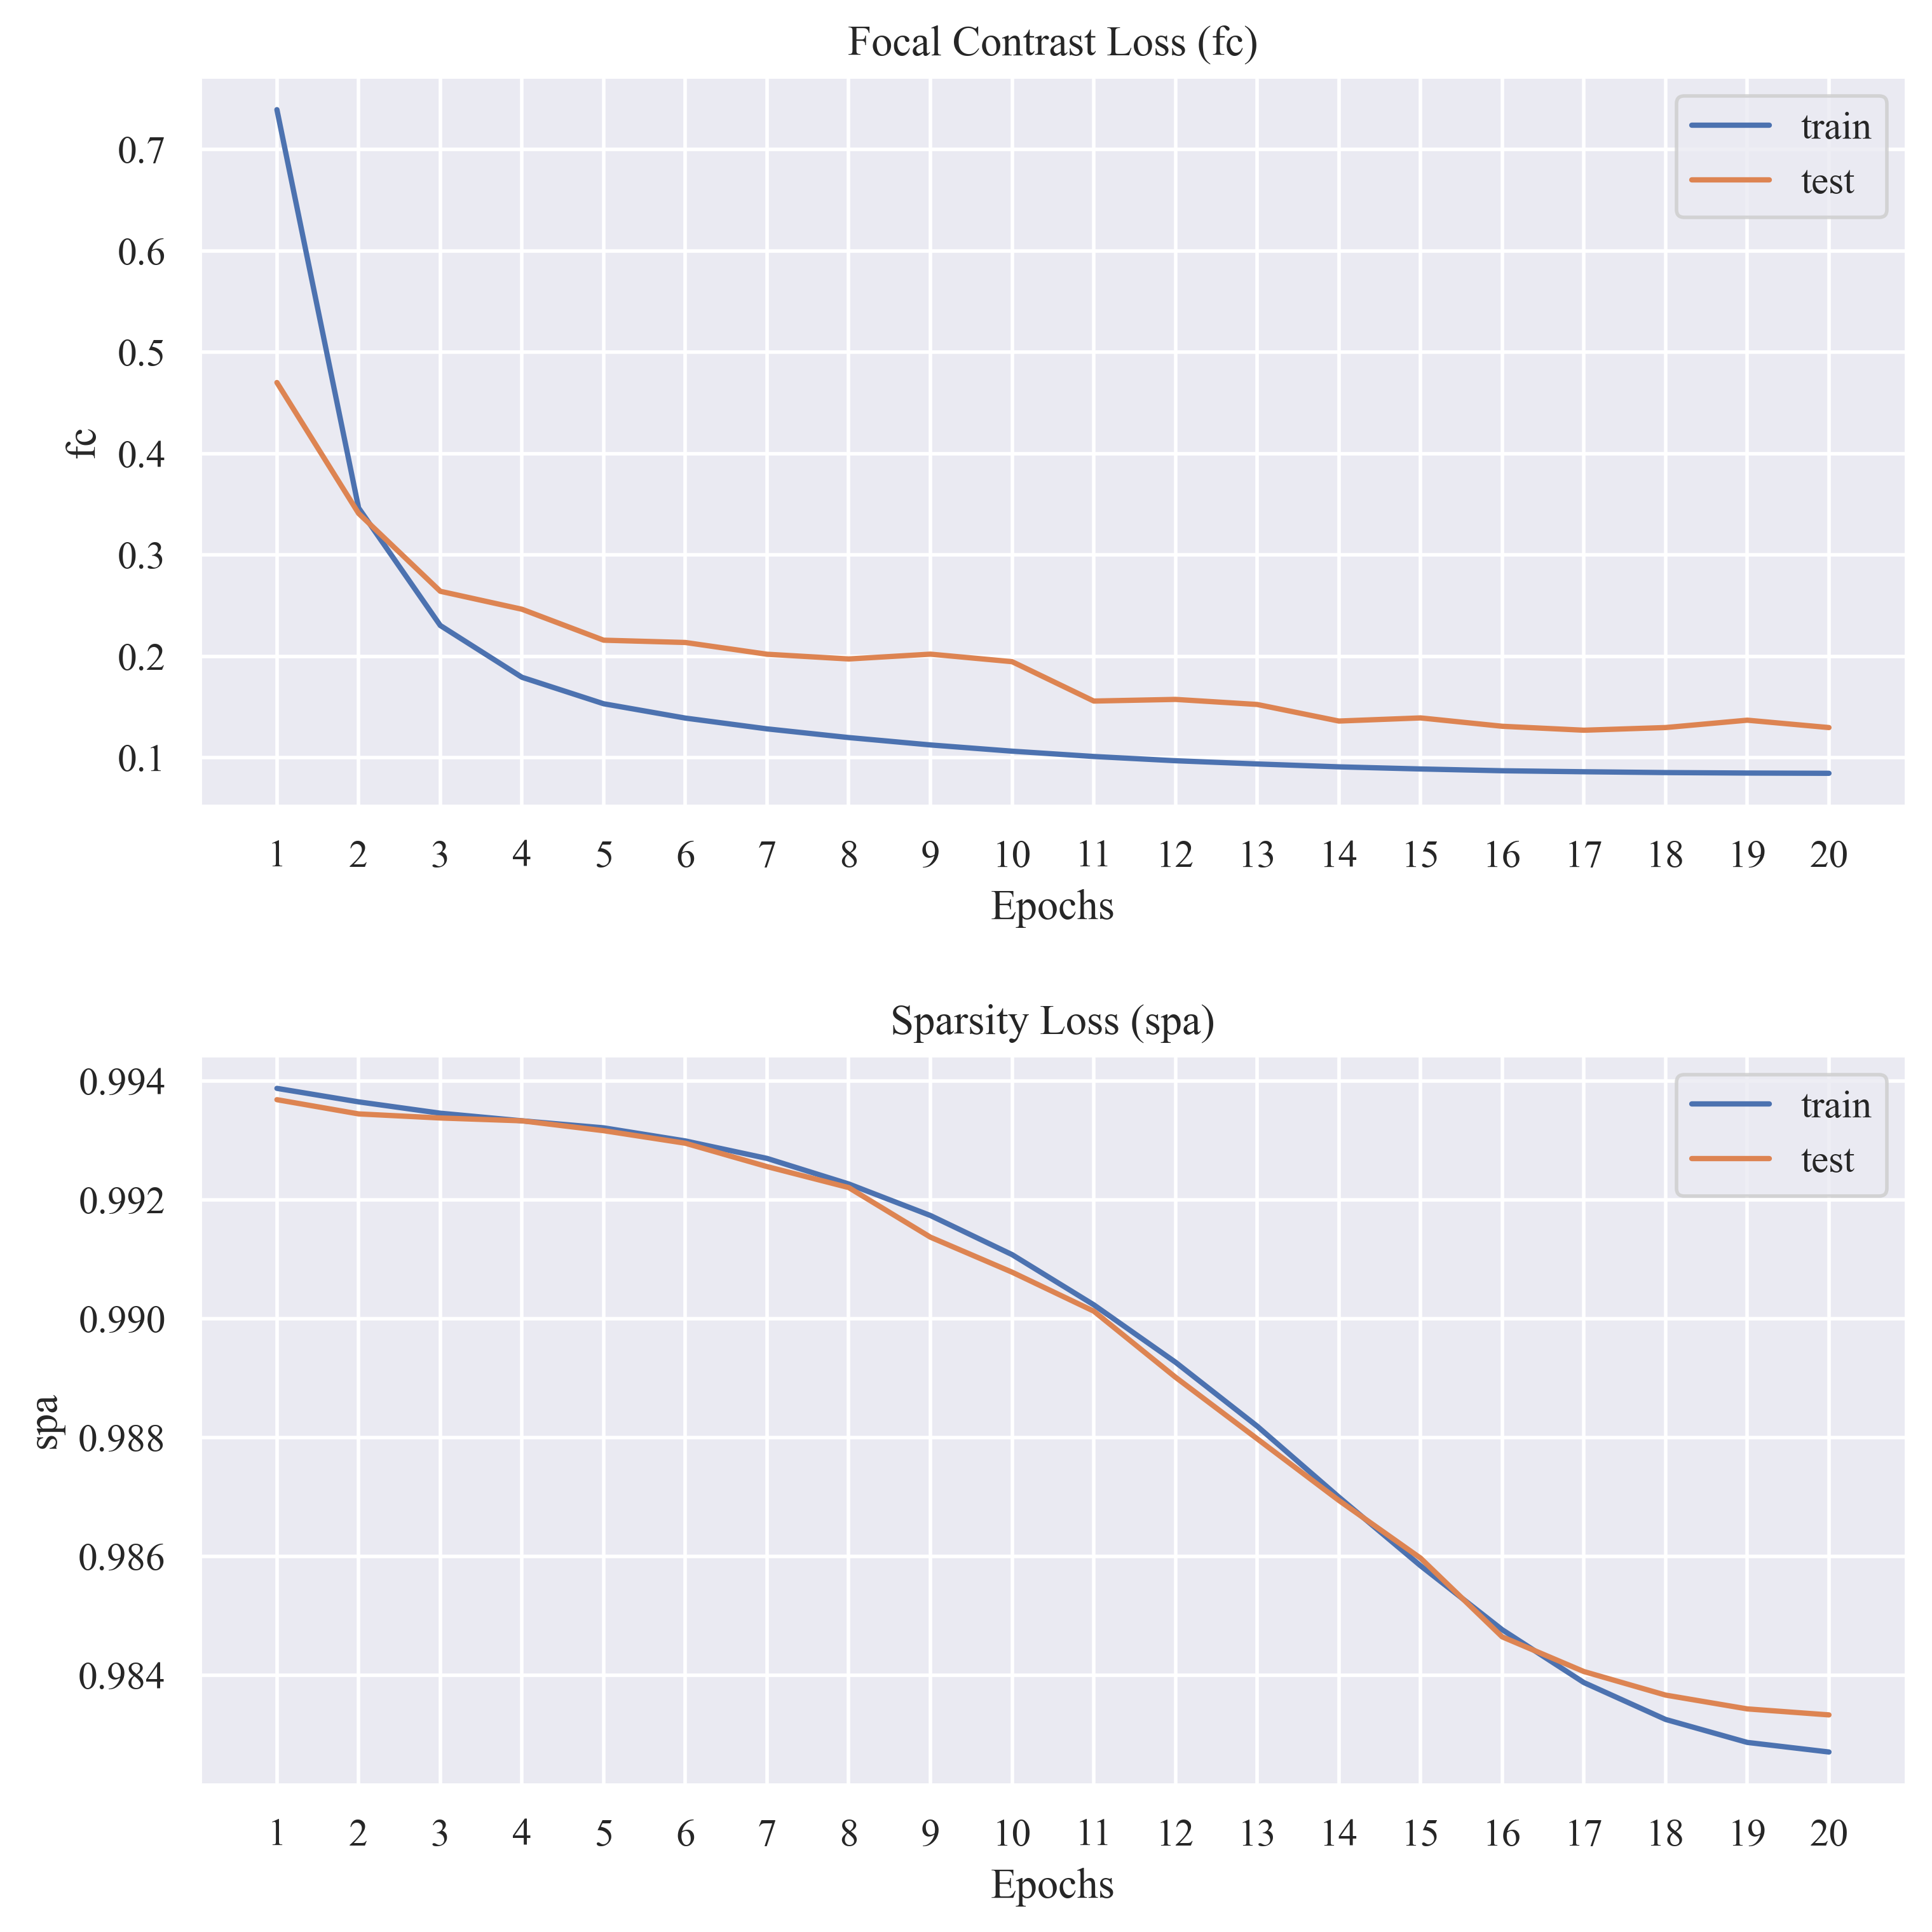
\includegraphics[scale=0.35]{figure/afloss.png}
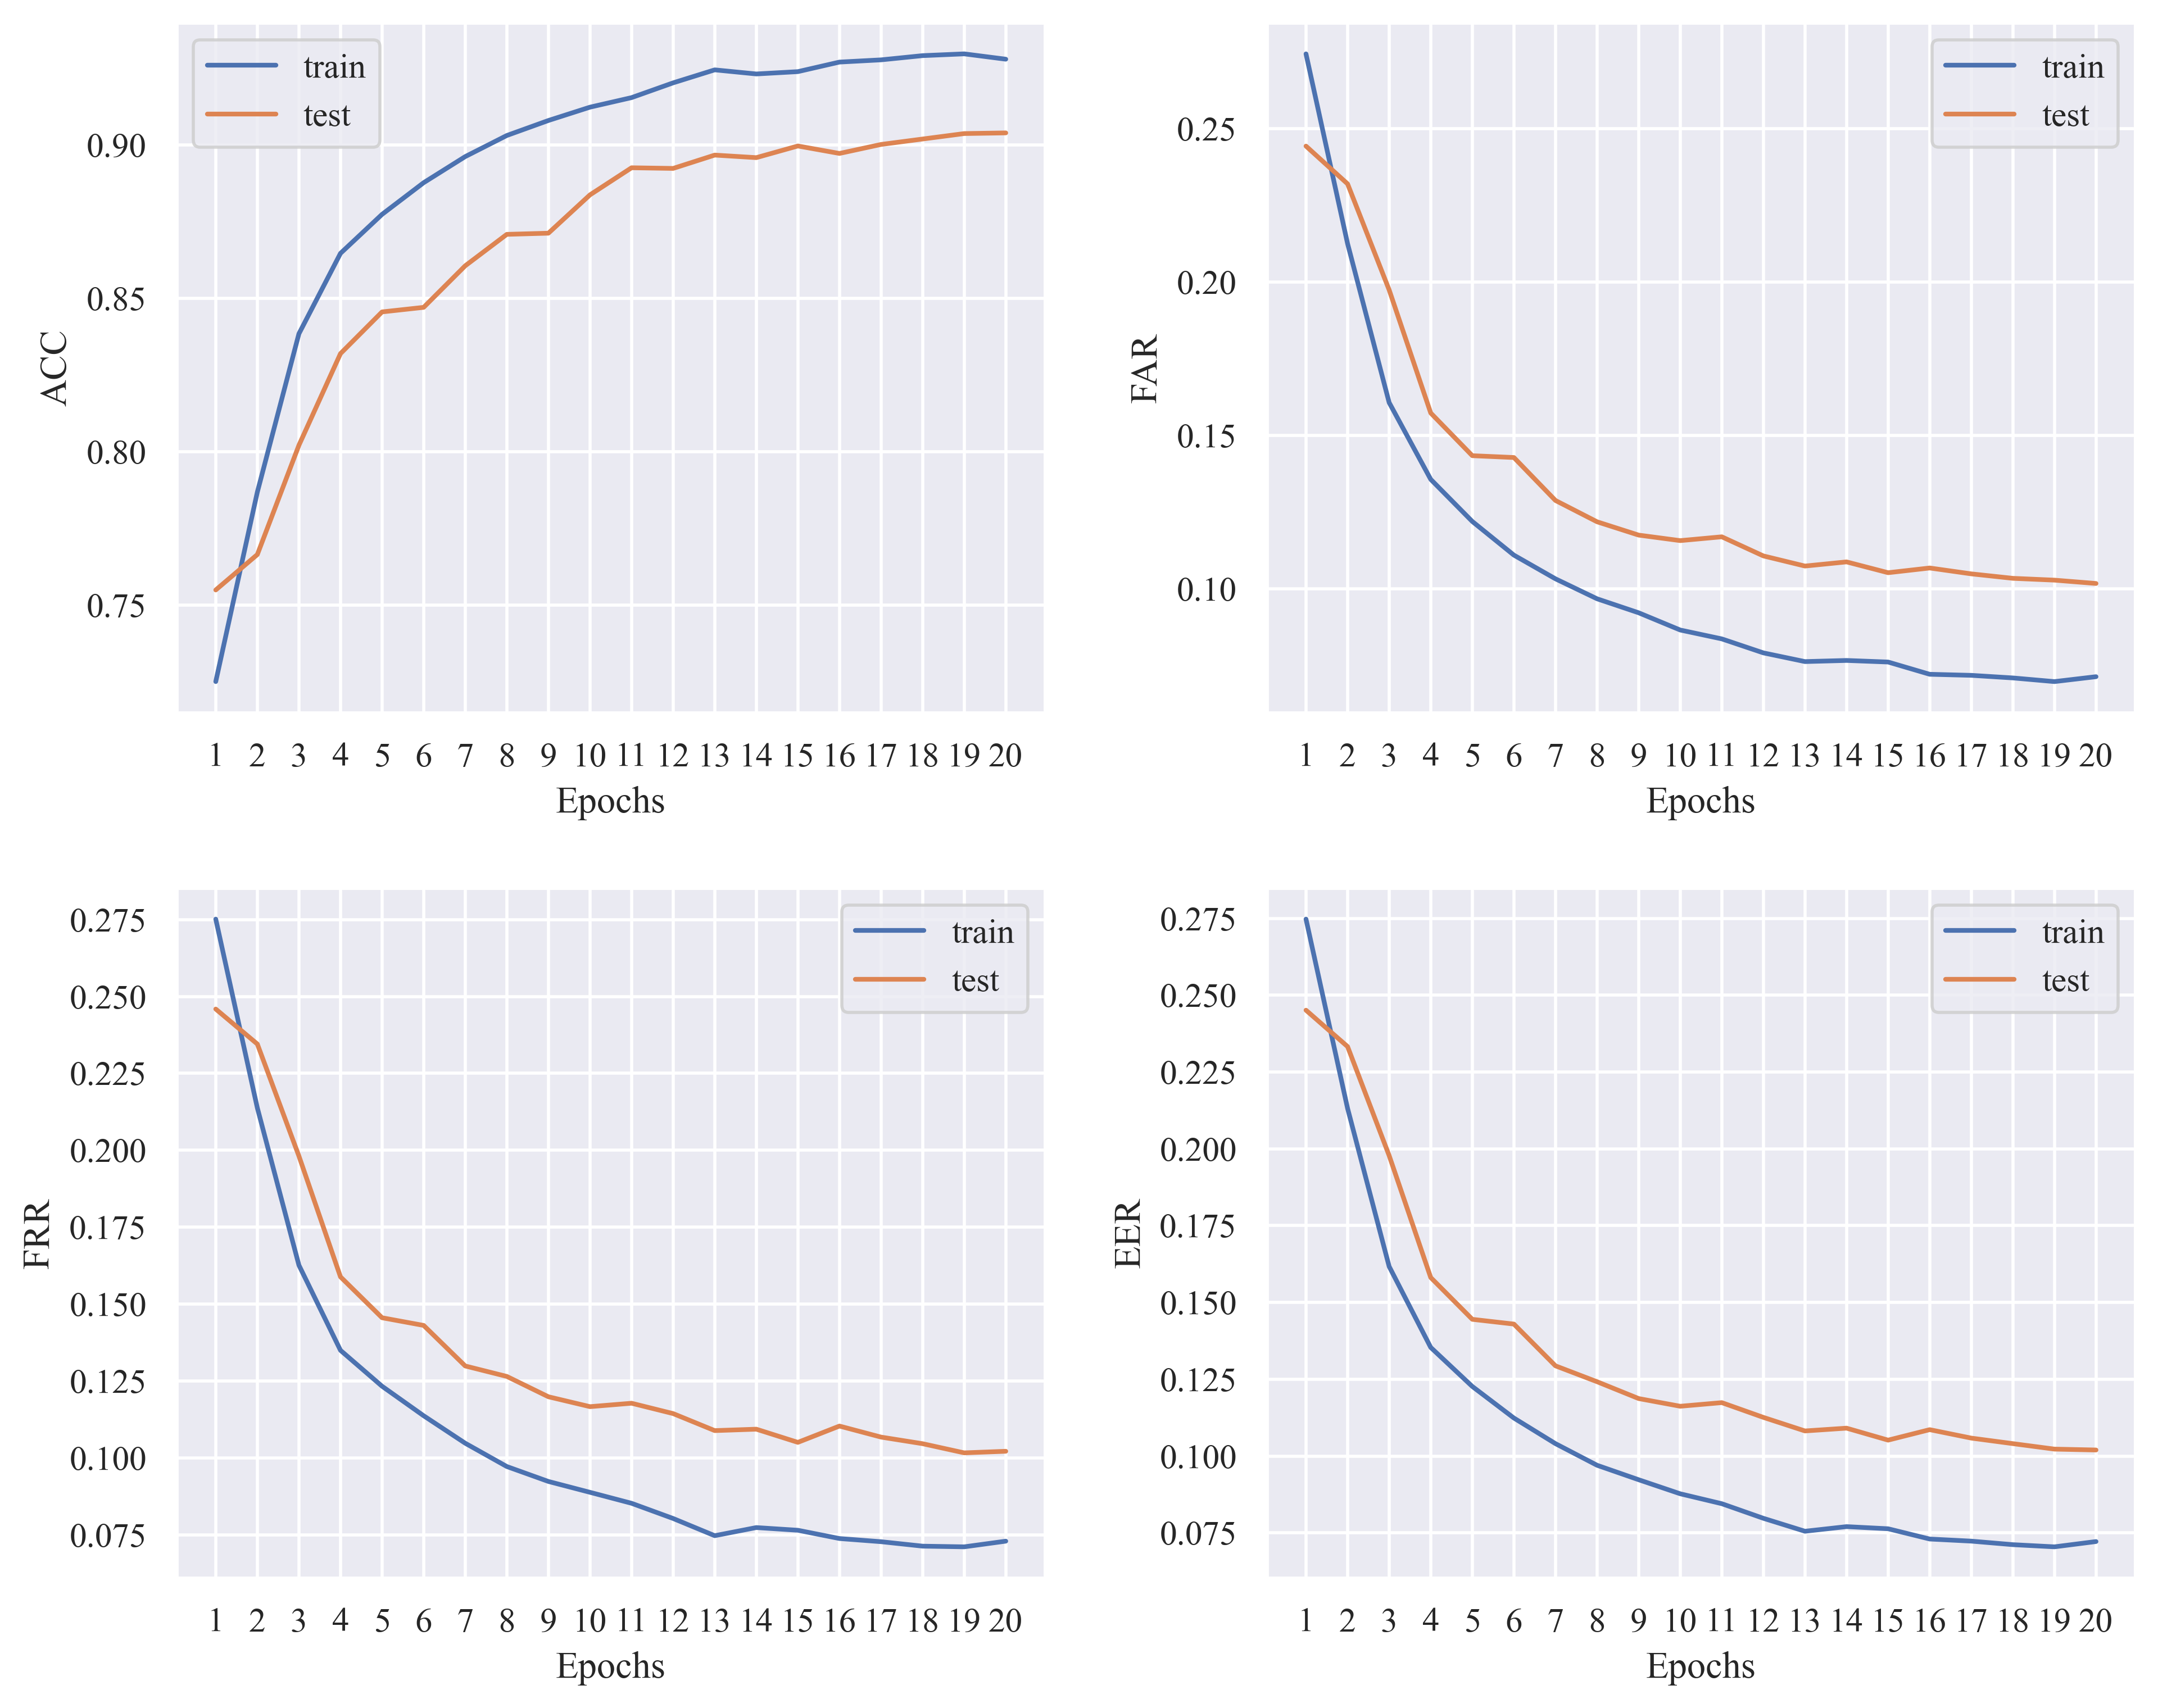
\includegraphics[scale=0.34]{figure/afmetrics.png}
\caption{Optimized Conv-Module loss and metrics diversification}
\label{fig:afloss}
\end{figure}

Based on the results, it can be found that the parameters of the pre-optimization OSVTF start converging at about the 7th or 8th Epoch in the proposed experimental scheme, while the parameters of the optimized OSVTF start converging at about the 3rd or 4th Epoch. This feature processing method of downsampling followed by mapping can effectively accelerate the convergence speed of the model training process. Since the number of features extracted from the intermediate network layer of OSVTF is large, this approach can learn the sensitive part of forged signature features more quickly, and combined with the computation of cross-multiple attention, it further strengthens the learning of the features of the sensitive part of the forged signature, and this approach can reduce a certain number of model parameters, which makes the size of the model weight file become smaller, and the inference speed is accelerated.

\chapter{Conclusions}
結論由研究結果引伸而來,相同的研究結果,不同的研究者可能引伸
出不同的結果,作者可表達對此結果具有的理論和實際價值的看法, 具體要求如下:

(1) 包括研究過程中所遇到或引發的種種現象思考、根據研究成果,提
出解決問題的方向,以及未來值得研究的方向。

(2) 結論要根據論文寫出總結性內容,觀點需具體明確,要有自己的創
見。

(3) 應直接回答研究問題。論據充分,層次清楚,觀點明確,要點分明,
評論合理可信。提示進一步研究的問題,交待本研究是否具體可行,
提示亟待改進之處,詳細地交待研究限制。建議應具參考價值。



Review the main research purpose or hypothesis, discuss whether the results meet the expectations, and briefly explain the reasons.

Summarize the main research results, discuss the consistency or inconsistency with other scholars' conclusions and the reasons.


Point out the limitations of the research and the possible impact of the limitations.

Point out the theoretical significance or potential engineering application value of the results.




%% -------------------------------------------------<< bib 參考文獻 中英文 bib 文件要分別創建

\bibreference


%% -------------------------------------------------<< 附錄
\MUSTappendix{
	
主要是冗長結論如定理的證明, 以及實驗中裝置的冗長描述及參數等。

\section*{A.1 An appendix}


% \subsection{List of symbol}

%  $G$ \hspace{12.5em} Deterministic finite automaton
%  $G_{nd}$ \hspace{11.8em} Nondeterministic finite automaton
%  $\delta$ \hspace{12.6em} Partial state transition function
%  $x_0$ \hspace{12.4em} Initial state
%  $X_0$ \hspace{12.3em} Set of initial states
%  $\Sigma$ \hspace{12.7em} Set of events
%  $\Sigma^{\ast}$ \hspace{12.3em} Set of sequences
%  $\Sigma_c$ \hspace{12.3em} Set of controllable events
%  $\Sigma_{uc}$ \hspace{12em} Set of uncontrollable events
%  $\Sigma_o$ \hspace{12.3em} Set of observable events
%  $\Sigma_{uo}$ \hspace{12em} Set of unobservable events
%  $\Sigma_f$ \hspace{12.3em} Set of fault events
%  $\emptyset$ \hspace{12.8em}   Empty set
%  $\varepsilon$  \hspace{12.8em} Empty sequence
%  $S$ \hspace{12.8em} Supervisor
%  $AT$ \hspace{12em} Attacked labels
%  $T_q$ \hspace{12.4em} Quiescent gross decision structure
%  $\Gamma$ \hspace{12.7em} Set of control actions
%  $X_S$ \hspace{12.3em} Set of secret states



% \subsection*{A.2~smithchart mirrored}
% \begin{figure}[H]
% 	\centering
% 	\begin{tikzpicture}[scale=1.2]
% 	\begin{smithchart}[smithchart mirrored,]
% 	\addplot coordinates {
% 		(0.5,0.2) (1,0.8) (2,2)
% 	};
% 	\end{smithchart}
% 	\end{tikzpicture}
	
% \end{figure}














% \subsection*{A.3~plot3D}
% \begin{figure}[H]

% 	\begin{subfigure}{.49\textwidth}
% 		\centering
% 		\begin{tikzpicture}[scale=0.7]
% 		\begin{axis}[
% 		xlabel={Temperature [\textcelsius]},
% 		ylabel={Solubility [g per 100 g water]},
% 		ymajorgrids=true,
% 		grid style=dashed,]
% 		\addplot[color=red]{exp(x)};
% 		\end{axis}
% 		\end{tikzpicture}
% 		\caption{A subfigure}
% 	\end{subfigure}
% %-----------------------------------------------------------
% 	\begin{subfigure}{.49\textwidth}
% 		\centering
% 		\begin{tikzpicture}[scale=.7]
% 			\begin{axis}[
% 				xlabel={Temperature [\textcelsius]},
% 				ylabel={Solubility [g per 100 g water]},
% 				xmin=0, xmax=100,
% 				ymin=0, ymax=120,
% 				xtick={0,20,40,60,80,100},
% 				ytick={0,20,40,60,80,100,120},
% 				legend pos=north west,
% 				ymajorgrids=true,
% 				grid style=dashed,
% 				]
% 				\addplot[
% 				color=blue,
% 				mark=square,
% 				]
% 				coordinates {
% 					(0,23.1)(10,27.5)(20,32)(30,37.8)(40,44.6)(60,61.8)(80,83.8)(100,114)
% 				};
% 				\legend{CuSO$_4\cdot$5H$_2$O}
% 			\end{axis}
% 		\end{tikzpicture}
% 		\caption{A subfigure}
% 	\end{subfigure}
% %-----------------------------------------------------------
% 	\centering
% 	\begin{subfigure}{.49\textwidth}
% 		\begin{tikzpicture}[scale=0.7]
% 			\begin{axis}[
% 				axis lines = left,
% 				xlabel = $x$,
% 				ylabel = {$f(x)$},
% 				ymajorgrids=true,
% 				grid style=dashed,]
% 				]
% 				%Below the red parabola is defined
% 				\addplot [
% 				domain=-10:10, 
% 				samples=100, 
% 				color=red,
% 				]
% 				{x^2 - 2*x - 1};
% 				\addlegendentry{$x^2 - 2x - 1$}
% 				%Here the blue parabloa is defined
% 				\addplot [
% 				domain=-10:10, 
% 				samples=100, 
% 				color=blue,
% 				]
% 				{x^2 + 2*x + 1};
% 				\addlegendentry{$x^2 + 2x + 1$}
% 			\end{axis}
% 		\end{tikzpicture}
% 		\caption{A subfigure}
% 	\end{subfigure}
% \end{figure}




% \subsection*{A.4~plot3D}
% \begin{figure}[H]
% 	\centering
% 	\begin{tikzpicture}[scale=1.2]
% 	\begin{axis}[
% 	hide axis,
% 	xlabel=$x$,ylabel=$y$,
% 	mesh/interior colormap name=hot,
% 	colormap/blackwhite,
% 	]
% 	\addplot3 [domain=-1.5:1.5,surf]
% 	{-exp(-x^2-y^2)};
% 	\end{axis}
% 	\end{tikzpicture}

% app:plot3D
% \end{figure}
}


%% -------------------------------------------------<< 致謝
\MUSTacknowledgement{
	First of all, I would like to express my ddep gratitude to Professor Xin Liu, my supervisor. She gave me a lot of encouragement during the research period, so that I could overcome the difficulties in researching difficult doubts, overcome psychological laziness, and constantly challenge and surpass myself. During the period from the topic selection report to the thesis, she provided many research perspectives and innovations, gave me many key suggestions during the research period, carefully examined the thesis and made relevant suggestions for modification, which enabled me to better improve the content of each part, and not only enabled me to acquire more knowledge, but also knew how to handle various details.

Secondly, I would like to thank the professors of the School of Innovative Engineering, who taught me all they could during these two years of study, allowing me to reconstruct my previous knowledge framework from a different perspective. The lectures also gave me a stage to show my personal ability, allowing me to learn new knowledge while practicing my presentation skills, and the English-focused lectures helped me to improve my English reading and writing skills to a certain extent.

Finally, I would like to thank my family for their support and help during the study period, which helped me to calmly think about the situation and find solutions from my own point of view at every critical moment, and also made me know that I should be calm in doing things, be a good listener when listening to others, and be an eloquent speaker when talking to others.




% I would like to express my deep gratitude to Professor xxx and
% Professor xxx, my research supervisors, for their patient
% guidance, enthusiastic encouragement and useful critiques of
% this research work.

% I would also like to extend my thanks to the technicians of the
% laboratory of the xxx department for their help in offering me the
% resources in running the program.
% Finally, I wish to thank my parents and brothers for their support
% and encouragement throughout my study.


}





%% -------------------------------------------------<< 個人簡歷
% 入學時間
\def\mustProfilea{
	2014.09
}


% 起止年月
\def\mustProfileb{
	2010.09--2014.06 \\
	2014.09--2017.06
}


% 就讀學校
\def\mustProfilec{
	X~X~X~大學 \\
	X~X~X~大學
}


% 取得學位名稱
\def\mustProfiled{
	X~X~學士學位\\
	X~X~碩士學位
}


%發表的學術論文、著作(論文/著作名稱、報刊/出版社名稱、發表時間、刊物/出版社級別)
\def\mustProfilee{
\smallskip
	待寫,待補
}


%參加的學術項目(項目名稱、項目時間、立項單位、承擔的工作)
\def\mustProfilef{
\smallskip
	待寫,待補
}



% 自動生成個人簡歷

\MUSTProfile



\end{document}



























% The English template was written by Tao Qin on April 3, 2022.